\documentclass[a4paper,twoside]{report}

\usepackage[T1]{fontenc}
\usepackage[polish]{babel}
\usepackage[utf8]{inputenc}
\usepackage{hhline}
\usepackage{hyperref}
\PassOptionsToPackage{hyphens}{url}
\usepackage{graphicx}
\usepackage{subfigure}
\usepackage{psfrag}
\usepackage{float}
\restylefloat{figure}

\usepackage{lmodern}
\usepackage{float}
\selectlanguage{polish}
\usepackage{amsmath}
\usepackage{amsfonts}
\usepackage{geometry}
\PassOptionsToPackage{hyphens}{url}
\usepackage{enumitem}
\setlist[description]{leftmargin=\parindent,labelindent=\parindent}

\newgeometry{tmargin=2cm, bmargin=2.5cm, lmargin=2.5cm, rmargin=2.5cm}
\renewcommand*\thesection{\arabic{section}} % zmiana numeracji sekcji 0.X -> X
\author{\textbf{KN EZI Team}}
\title{Opracowanie pytań do obrony (EZI)}
\frenchspacing

\begin{document}
\maketitle
%\bigskip 
\tableofcontents %spis tresci
\thispagestyle{empty}
\newpage

%\part{Zagadnienia specjalnościowe}
\bigskip
\section{Sterowniki mikroprocesorowe i ich zastosowania}

Główną częścią takiego sterownika jest mikrokontroler pełniący funkcję jednostki wykonującej operacje logiczne i arytmetyczne.

\subsection{Sterownik PLC}

\paragraph{Programowalny sterownik logiczny PLC} (ang. Programmable Logic Controller) uniwersalne urządzenie mikroprocesorowe przeznaczone do sterowania pracą maszyny lub urządzenia technologicznego. Sterownik PLC musi zostać dopasowany do określonego obiektu sterowania poprzez wprowadzenie do jego pamięci żądanego algorytmu działania obiektu - zaprogramowanie go. Cechą charakterystyczną sterowników PLC odróżniającą ten sterownik od innych sterowników komputerowych jest cykliczny obieg pamięci programu. Algorytm jest zapisywany w dedykowanym sterownikowi języku programowania. Istnieje możliwość zmiany algorytmu przez zmianę zawartości pamięci programu. Sterownik wyposaża się w odpowiednią liczbę układów wejściowych zbierających informacje o stanie obiektu i żądaniach obsługi oraz odpowiednią liczbę i rodzaj układów wyjściowych połączonych z elementami wykonawczymi, sygnalizacyjnymi lub transmisji danych. Układy I/O mogą być cyfrowe lub analogowe.

Zasada działania: przeglądanie wejść i w zależności od ich stanu oraz
wprowadzonego programu użytkownika ustawianie stanu wyjść dwustanowych (zał/wył).
PLC jest w swej istocie komputerem przemysłowym ze specjalnie zaprojektowaną jednostką centralną oraz rozbudowanymi układami wejść/wyjść do kontaktu z zewnętrznymi urządzeniami przemysłowymi (urządzeniami polowymi). Wcześniej działanie sterowników były realizowane przy pomocy rozbudowanej sieci elektrycznej przy zastosowaniu przekaźników.

\subsubsection{Historia}
Inżynierowie z Hydramatic Division firmy GM w roku 1968 sformułowali założenia dla sterownika programowalnego, którego główna zaletą miała być redukcja wysokich kosztów związanych z niewielką elastycznością systemów przekaźnikowych. W 1969 r. został opracowany pierwszy sterownik PLC.

\subsubsection{Założenia sterownika}
\begin{itemize}
\item realizacja na urządzeniach półprzewodnikowych,
\item elastyczność komputera,
\item praca w środowisku przemysłowym (wibracje, wysoka temperatura, zapylenie itp.),
\item możliwość przeprogramowywania,
\item łatwe programowanie i obsługa przez elektryków i techników.
\end{itemize}

\subsubsection{Budowa}
\begin{itemize}
\item jednostka centralna (CPU),
\item zasilacz,
\item pamięć,
\item układy I/O,
\item port komunikacyjny (np. PROFIBUS),
\item gniazdo rozszerzenia.
\end{itemize}

\subsubsection{Języki programowania}
\begin{itemize}
\item \textbf{drabinkowy LD} (ang. Ladder Diagram) - logika drabinkowa, a schemat podobny do klasycznego rysunku technicznego elektrycznego,
\item \textbf{blokowy FBD} (ang. Function Block Diagram) - diagram bloków funkcyjnych, sekwencji linni zawierająca te bloki,
\item \textbf{strukturalny ST} (ang. Structured Text) - tekst strukturalny - język zbliżony do Pascala;
\item \textbf{lista instrukcji IL} (ang. Instruction List) lista instrukcji - rodzaj asemblera,
\item \textbf{sekwencyjny SFC} (ang. Sequential Function Chart) sekwencyjny ciąg bloków - sekwencja bloków programowych z warunkami przejścia.
\end{itemize}

\subsection{Poziomy sygnałów}
\begin{itemize}
\item analogowe
	\begin{itemize}
	\item 0 ... 20 mA
	\item 4 ... 20 mA (najczęściej)
	\item 0 ... 5, 10 V
	\item -10 ... 10 V
	\end{itemize}
\item cyfrowe
	\begin{itemize}
	\item 5, 12, 24, 48 VDC
	\item 24, 128, 240 VAC
	\end{itemize}
\end{itemize}
Źródłami sygnałów analogowych są: termometry, przepływomierze, wilgotnościomierze, mierniki nacisku, potencjometry.

Analogowe sygnały wejściowe sterują: zaworami analogowymi, szybkością obrotów silników, rejestratorami.

\subsection{Zadania PLC}
\begin{itemize}
\item skanowanie wejść,
\item wykonywanie instrukcji,
\item ustawianie wyjść,
\item samodiagnostyka.
\end{itemize}

\subsection{Regulator PID}

\paragraph{Regulator PID} (ang. Proportional-Integral-Derivative controller) – regulator stosowany w układach regulacji składający się z trzech członów: proporcjonalnego, całkującego i różniczkującego. Najczęściej jego celem jest utrzymanie wartości wyjściowej na określonym poziomie, zwanym wartością zadaną. Jest najczęściej stosowanym regulatorem w przemyśle.\\

Właściwości  dynamiczne  idealnych  regulatorów  PID  mogą  być  opisane  za  pomocą transmitancji operatorowej, będącej stosunkiem transformaty Laplace’a sygnału wyjściowego regulatora U’(s) i transformaty Laplace’a uchybu regulacji (sygnału wejściowego) E(s):
\begin{equation}
G_r(s)=\dfrac{U'(s)}{E(s)} = k_p(1+\dfrac{1}{T_i \cdot s}+ T_d \cdot s),
\label{wzor:PID_idealny}
\end{equation}
gdzie: \\
$k_p$ - wzmocnienie członu proporcjonalnego,\\
$T_i$ - czas całkowania (zdwojenia),\\
$T_d$ - czas różniczkowania (wyprzedzenia).\\

\begin{figure}[htbp]
\centering
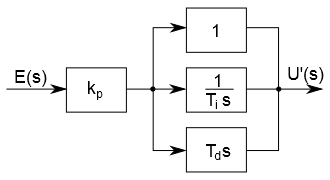
\includegraphics[scale=0.7]{obrazy/PID_blok.png}
\caption{Schemat blokowy idealnego regulatora PID}
\label{rys:PID_blok}
\end{figure}

\begin{figure}[htbp]
\centering
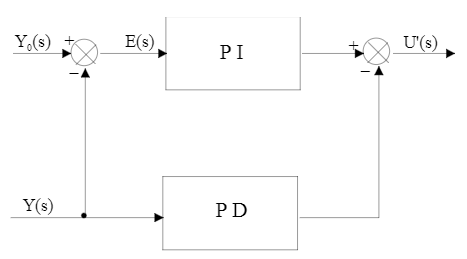
\includegraphics[scale=0.8]{obrazy/PID_uC_blok.png}
\caption{Schemat blokowy mikroprocesorowego regulatora PID}
\label{rys:PID_uC_blok}
\end{figure}

\paragraph{Zakres  proporcjonalności} $X = (1/k_p) \cdot 100 \%$ jest  to  procentowa  część  pełnego  zakresu zmian wielkości wejściowej e, potrzebna do wywołania pełnej zmiany wielkości wyjściowej u’ regulatora.

\paragraph{Czas zdwojenia (całkowania)} $T_i$ dotyczy regulatorów PI, których wielkość wyjściowa ma zarówno  składową  proporcjonalną $u_p$,  jak  i  całkującą $u_i$.  Czas  zdwojenia  określa  się  na podstawie znajomości charakterystyki czasowej skokowej regulatora. Jest to czas potrzebny na  to,  aby sygnał  wyjściowy  regulatora,  będący  wynikiem  działania  całkującego,  stał  się równy sygnałowi będącemu wynikiem działania proporcjonalnego (rysunek \ref{rys:czas_zdwojenia}.).

\begin{figure}[htbp]
\centering
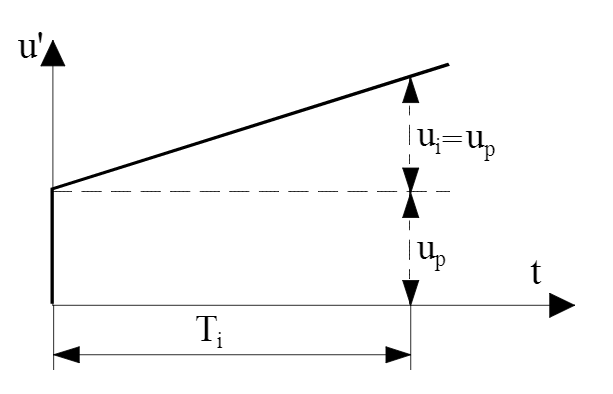
\includegraphics[scale=0.4]{obrazy/czas_zdwojenia.png}
\caption{Sposób wyznaczania czasu zdwojenia Ti}
\label{rys:czas_zdwojenia}
\end{figure}

Zatem sygnał wyjściowy z regulatora PI (wypadkowy  dla obu oddziaływań) po czasie $T_i$ zwiększa dwukrotnie swoją wartość. Stąd pochodzi jego nazwa – czas zdwojenia.  

\paragraph{Czas  wyprzedzenia  (różniczkowania)} $T_d$ dotyczy  regulatorów  PD,  których  wielkość wyjściowa ma zarówno składową proporcjonalną, jak i różniczkującą. Czas wyprzedzenia określa  się  na  podstawie  odpowiedzi  regulatora  na  wymuszenie  w  postaci  narastającego liniowo sygnału uchybu regulacji e. Jest  to czas, po którym sygnał wyjściowy regulatora, związany  zdziałaniem  proporcjonalnym $u_p$,  zrówna  się  z  sygnałem  pochodzącym  od działania różniczkującego $u_d$ (rysunek \ref{rys:czas_wyprzedzenia}.).

\begin{figure}[htbp]
\centering
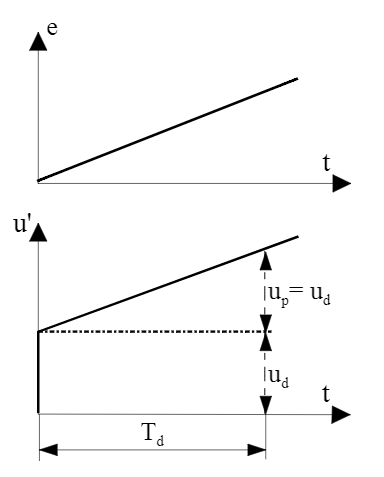
\includegraphics[scale=0.5]{obrazy/czas_wyprzedzenia.png}
\caption{Sposób wyznaczania czasu wyprzedzenia Td}
\label{rys:czas_wyprzedzenia}
\end{figure}

Wielkości $k_p$ (w starszych typach regulatorów X), $T_i$ i $T_d$ noszą nazwę nastaw regulatora. Są to parametry nastrajalne, które dobieramy tak, aby:
\begin{itemize}
\item uzyskać odpowiednie własności dynamiczne regulatora,
\item uzyskać najlepszą jakość regulacji.
\end{itemize}

Transmitancja określona wzorem \eqref{wzor:PID_idealny} dotyczy regulatora idealnego, którego w praktyce nie daje  się  zrealizować.  W  warunkach  rzeczywistych  w  członie  różniczkującym  występuje inercja, określona stałą czasową T. Stała ta nie jest nastawialna. Zatem zamiast członu~$T_d \cdot s$ w transmitancji  występuje  człon~$T_ds/Ts+1$. Transmitancja  operatorowa  rzeczywistego  regulatora PID ma wówczas postać:
\begin{equation}
G_r(s)=\dfrac{U'(s)}{E(s)} = k_p(1+\dfrac{1}{T_i \cdot s}+ \dfrac{T_d \cdot s}{T s + 1}),
\end{equation}

\subsection{Sterownik CNC}
\paragraph{Sterownik CNC} (ang. Computer Numerical Control) to typ sterownika mikroprocesorowego, który programuje się za pomocą tzw. G code'u. Sterowniki te używane są m.in. do kontroli takich urządzeń jak: frezarki, tokarki a w szerszym zastosowaniu do sterowania robotami fabrycznymi, które pracują w tzw. trybie taśmy montażowej np. automaty składające podzespoły samochodowe.

W nowoczesnych maszynach CNC stosuje się sterowniki pracujące na bazie komputera przemysłowego IPC w technologii ,,PC-based Automation''. W tej technologii sterownik CNC działa programowo, a nie sprzętowo, tak jak to odbywało się w starego typu dedykowanych sterownikach. System operacyjny czasu rzeczywistego sterownika, realizuje funkcje PLC, HMI i sterowania ruchem, odpowiadając za funkcjonalność całej maszyny.

\subsection{Kontroler PAC}
\paragraph{Sterowniki PAC} (ang.Programmable Automation Controller) zwane sterownikami automatyki są dużymi systemami sterownikowymi przeznaczonymi do obsługi złożonych procesów technologicznych. Wiele dotychczasowych sterowników PLC o największej wydajności zostało nazwanych przez producentów sterownikami PAC. Granica pomiędzy dużymi i wydajnymi sterownikami PLC a sterownikami PAC jest obecnie słabo widoczna.
Współczesne procesy sterowania wykorzystują ogromne ilości sygnałów i danych, począwszy od analogowych i cyfrowych urządzeń wejścia/wyjścia, poprzez szybkie kamery wysokiej rozdzielczości, a kończąc na wieloosiowych
sterownikach ruchu. Takie zastosowania, jak: szybka produkcja, monitoring pracy maszyn w czasie rzeczywistym, sterowanie precyzyjne czy sterowanie złożonym procesem, wymagają deterministycznych systemów akwizycji, zaawansowanej analizy i algorytmów przetwarzania danych.Wyższej klasy sterowniki PLC w pewnym stopniu spełniają te wymagania. Jednakże do wydajnego przetwarzania tych danych trzeba zastosować odpowiednie środki informatyczne, m.in. procesory zmiennoprzecinkowe i duże zasoby pamięci. Sterowniki PAC integrują tego rodzaju gotowe składniki sprzętowe w ramach systemu czasu rzeczywistego, oferując w ten sposób wydajną platformę dla inżynierów automatyki.

\section{Lokalne sieci komputerowe}
\paragraph{Sieci lokalne LAN} (ang. Local Area Network), są sieciami prywatnymi obejmującymi pojedynczy budynek lub grupę budynków w obszarze o średnicy do kilku kilometrów. Sieci te są powszechnie używane do łączenia komputerów osobistych i stacji roboczych w biurach firmy i fabrykach w celu udostępnienia zasobów (np. drukarek) i wymiany informacji. 

Sieci LAN od innych typów odróżniają trzy cechy:
\begin{itemize}
\item rozmiary,
\item technologie transmisji,
\item topologia.
\end{itemize}

Sieci LAN mają ograniczone rozmiary, co oznacza, że czas przesyłu w najgorszym przypadku jest ograniczony i z góry znany.

Sieci lokalne mogą korzystać z technologii transmisji opartej na kablu lub technologii bezprzewodowej. Tradycyjne sieci LAN charakteryzują się szybkością przesyłu od 10 Mb/s do 100 Mb oraz niskim opóźnieniem. Nowsze sieci lokalne działają z szybkością do 10 Gb/s. 

W rozgłoszeniowych sieciach LAN możliwe są różnorodne topologie. Przykładem jest sieć magistralowa (zbudowana z kabla liniowego). W sieci magistralowej, w każdej chwili najwyżej jedno urządzenie jest nadrzędne i ma prawo do nadawania. Potrzebny jest zatem mechanizm arbitrażu który rozstrzyga konflikt gdy dwa lub więcej urządzeń chce nadawać jednocześnie. Mechanizm arbitrażu może być scentralizowany lub rozproszony. Na przykład sieć Ethernet jest siecią rozgłoszeniową opartą na magistrali ze zdecentralizowanym sterowaniem. Komputery w tej sieci mogą nadawać w dowolnej chwili. W razie kolizji dwóch lub więcej pakietów każdy komputer oczekuje losowy odstęp czasu i ponawia próbę. Drugim typem systemu rozgłoszeniowego jest pierścień. W pierścieniu każdy bit propaguje się samodzielnie bez czekania na resztę pakietu, do którego należy. Zazwyczaj każdy bit okrąża cały pierścień w czasie potrzebnym na transmisję kilku bitów, często zanim komplety pakiet zostanie wysłany.
\section{Bazy danych i ich zastosowania}

\paragraph{Baza danych} - zbiór danych zapisanych zgodnie z określonymi regułami. W węższym znaczeniu jest to program (system) służący do zbierania, przetwarzania i organizowania informacji. 
Bazy danych pozwalają przechowywać dowolne informacje, na przykład informacje o ludziach, produktach czy zamówieniach. Dla systemów komputerowych mogą to być dane numeryczne, tekstowe, binarne, daty, lub inne dostępne typy w danym systemie. Można więc przechowywać grafikę, muzykę - np. jako pliki binarne. Kartoteka w bibliotece to również baza danych.
 Za bazę danych uważany może być plik tekstowy, arkusz kalkulacyjny, plik binarny. Gdy ilość danych rośnie, powstają nadmiarowe i niespójne dane. Dlatego wprowadza się różne systemy bazodanowe umożliwiające łatwiejsze zarządzanie dużą ilością danych - np. MS SQL, MySQL, Access.
 
Z uwagi na cenę danych współczesne systemy bazodanowe stanowią  podstawą działalności wielu firm, co wymaga istnienia możliwie niezawodnych systemów baz danych. \\
\textbf{System zarządzania bazą danych} - oprogramowanie umożliwiające tworzenie oraz eksploatację bazy danych oraz jej użytkowników. \\
\textbf{baza danych} = dane + schemat bazy danych (np. relacyjny) \\
\textbf{system bazy danych} = baza danych + system zarządzania bazą
\medskip 


\subsubsection{Kryteria klasyfikacji baz danych}
\begin{itemize}
\item Wielkość
\item Liczba odwołań
\item Stopień ważności informacji
\item Struktura informacji
\item Implementacja komputerowa
\end{itemize}
Bazy danych można podzielić według struktur organizacji danych, których używają:
\begin{itemize}
\item Bazy proste: kartotekowe, hierarchiczne (struktura drzewa, np katalogi w systemie)
\item Bazy złożone: relacyjne, obiektowe, relacyjno-obiektowe, strumieniowe, temporalne, nierelacyjne (NoSQL), grafowe
\end{itemize}
Z wymienionych struktur, w praktyce zdecydowanie najczęściej używane są bazy relacyjne.
\medskip


\subsection{Bazy relacyjne}
Relacyjny model danych został zaproponowany w latach 70. Zaimplementowany w latach 80. 

Opiera się on na pojęciu relacji. Dane grupowane są w relacje reprezentowane przez tablice. Czyli tablica STUDENCI zawierająca wiersze (krotki) z danymi studentów (imię, indeks - kolumny) o odpowiednich typach - całość tworzy relację.
W modelu obiektowym relacji odpowiada obiekt. \\

\begin{figure}[htbp]
	\centering
	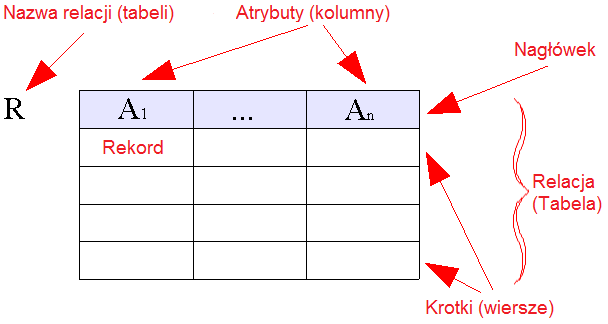
\includegraphics[scale=0.7]{obrazy/bazy/Relational_model_concepts_PL.png}
	\caption{Relacja}
\end{figure}
\subsubsection{Pojęcia}
\begin{itemize}
	\item \textbf{Klucz podstawowy (główny)} - najkrótszy zbiór atrybutów (czyli kolumn) pozwalający na \textbf{jednoznaczną} identyfikację wiersza w tabeli. Max 1 na tabelę.
	\item \textbf{Klucz obcy} - kolumna zawierająca wartości wskazujące na \textit{klucz główny} w innej tabeli, pozwala stworzyć związek pomiędzy tabelami. Typy związków: jeden do jednego, jeden do wielu, wiele do wielu (najczęściej realizowane za pomocą tabeli pośredniej).
\end{itemize}
Związki pomiędzy relacjami pozwalają uniknąć nadmiarowości danych i pozwalają zapewnić ich spójność. Jeżeli np. mamy tabelę studenci i samochody, relacja wiele do jednego (każdy samochód posiada klucz obcy czyli np. indeks studenta). Jeden student może posiadać więc wiele samochodów. Jeżeli chcemy sprawdzić czyj jest dany samochód to mamy klucz obcy studenta, a nie jego wszystkie dane - czyli wystarczy raz wpisać studenta, a zmiana jego danych następuje tez w jednym miejscu. Czyli minimalna ilość danych zapewnia spójność. Zły przypadek - tabela samochody zawiera wszystkie dane studenta, on zmienia imię, trzeba aktualizować dane we wszystkich jego samochodach (i pewnie o którymś się zapomni).\\\\
Zasady projektowania schematów relacyjnych baz danych opisują \textbf{zasady normalne}, najważniejsze:
\begin{description}
\item[1NF] Atrybuty są atomowe (niepodzielne) - kolumna [imię,nazwisko] - należy rozdzielić na 2 osobne kolumny, jedna komórka zawiera jedną wartość, czyli nie chcemy kolumny imiona.
\item[2NF] Każda kolumna niekluczowa zależy funkcyjnie od całego klucza głównego.
\item[3NF] Każda komórka w wierszu zależy jedynie od klucza głównego, \\
\lbrack indeks\rbrack, \lbrack imię\rbrack], \lbrack płeć\rbrack  \\
Zakładając że indeks to klucz główny, a płeć jest jednak związana z imieniem to ta ka tabela nie spełni tego wymagania, należy wydzielić drugą tabelę imiona: [imię], [płeć] a studentowi zostawić indeks i klucz obcy do tabeli imiona
\end{description}

Do pracy z relacyjnymi bazami danych służy \textbf{SQL} - standardowy język zapytań, używany do tworzenia, modyfikowania baz danych oraz do umieszczania i pobierania danych z baz danych.
Konkretnie: selekcje, projekcje, złączanie, usuwanie, modyfikację dodawania danych, a także operacje na schematach bazy danych - tworzenie, modyfikowanie tabel. \\
Zawiera on typy danych, umożliwia tworzenie funkcji, procedur składowanych.


\subsection{Z Wikipedii (takie powtórzenie)}
Relacyjne bazy danych (jak również przeznaczony dla nich standard SQL) oparte są na kilku prostych zasadach:

\begin{enumerate}
\item Wszystkie wartości danych oparte są na prostych typach danych.
\item Wszystkie dane w bazie relacyjnej przedstawiane są w formie dwuwymiarowych tabel (w matematycznym żargonie noszących nazwę ,,relacji''). Każda tabela zawiera zero lub więcej wierszy (w tymże żargonie – ,,krotki'') i jedną lub więcej kolumn (,,atrybutów''). Na każdy wiersz składają się jednakowo ułożone kolumny wypełnione wartościami, które z kolei w każdym wierszu mogą być inne.
\item Po wprowadzeniu danych do bazy, możliwe jest porównywanie wartości z różnych kolumn, zazwyczaj również z różnych tabel, i scalanie wierszy, gdy pochodzące z nich wartości są zgodne. Umożliwia to wiązanie danych i wykonywanie stosunkowo złożonych operacji w granicach całej bazy danych.
\item Wszystkie operacje wykonywane są w oparciu o algebrę relacji, bez względu na położenie wiersza tabeli. Nie można więc zapytać o wiersze, gdzie (x=3) bez wiersza pierwszego, trzeciego i piątego. Wiersze w relacyjnej bazie danych przechowywane są w porządku zupełnie dowolnym – nie musi on odzwierciedlać ani kolejności ich wprowadzania, ani kolejności ich przechowywania.
\item Z braku możliwości identyfikacji wiersza przez jego pozycję pojawia się potrzeba obecności jednej lub więcej kolumn niepowtarzalnych w granicach całej tabeli, pozwalających odnaleźć konkretny wiersz. Kolumny te określa się jako ,,klucz podstawowy'' (ang. primary key) tabeli.
\end{enumerate}

\subsection{Architektura Oracle}

\begin{figure}[htbp]
\centering
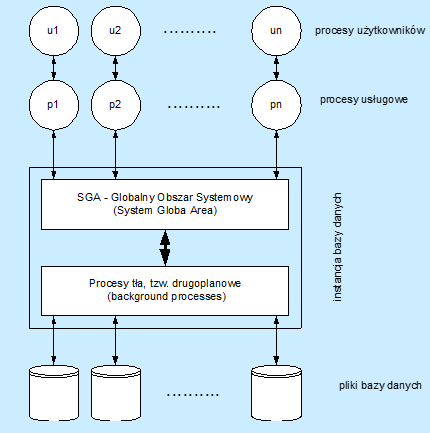
\includegraphics[scale=0.7]{obrazy/archoracle.png}
\caption{Architektura systemu}
\end{figure}


\medskip 
\paragraph{Rodzaje plików}

\begin{itemize}
\item pliki konfiguracyjne (init files) — najważniejszy z nich to plik parametrów (tzw. parameter file, w skrócie pfile) o nazwie init<SID>.ora, gdzie <SID> to unikalny (najczęściej 4-literowy) identyfikator instancji na danej maszynie, plik jest tekstowy i zawiera informacje o ustawieniach przy starcie bazy, a także o nazwie i położeniu plików kontrolnych
\item pliki kontrolne (control files) — binarne, bardzo ważne, zawierają informacje o położeniu WSZYSTKICH plików bazy danych wraz z datą i godziną ich zamknięcia
\item pliki danych (data files) — przechowują dane w postaci binarnej, z danych w nich zawartych korzysta się za pośrednictwem procesów serwera (tła)
\item  pliki dziennika powtórzeń (redo-log files) - rejestrują wszystkie operacje wykonane na bazie (na wypadek awarii), mogą być aktywne lub zarchiwizowane 
\item pliki śladu (trace files) — zawierają informacje o uszkodzeniach i o błędach procesów tła oraz procesów użytkowników
\item pliki kodu (code files) — wszelkie kody źródłowe, skrypty SQL itp 
\end{itemize}


\textbf{SGA} (ang. System Global Area). 
Składa się z:
\begin{itemize}
\item bufora danych, który:
Zawiera dane załadowane z dysku, okresowo zapisane (Dirty blocks), przechowuje informacje o zmianach, ma strukturę cykliczną.
\item bufora dziennika powtórzeń, który przechowuje informację o zmianach, ma strukturę cykliczną.
\item obszaru współdzielonego
\end{itemize}

\paragraph{Procesy tła}
\begin{itemize}
\item DBWR — database writer — zapisuje DIRTY BLOCKS na dysk 
\item LGWR — log writer — zapisuje zmiany do loga
\item CKPT — checkpoint — sygnalizuje tzw. punkt kontrolny + aktualizuje nagłówki plików kontrolnych
\item SMON — system monitor — odtwarza instancję, scala wolne obszary na dysku
\item PMON — process monitor — zwalnia zasoby procesu użytkownika, który się ,,zawiesił''
\item ARCH — archiwizator — opcjonalny, spowalnia pracę, umożliwia skonfigurowanie serwera lustrzanego
\end{itemize}

\paragraph{Stany bazy danych}

\begin{itemize}
\item IDLE - nieczynna, pliki zamknięte, procesy tła nie działają 
\item NOMOUNT - stan po odczytaniu pfile-a, zainicjowaniu SGA i uruchomieniu procesów tła, stan służący do tworzenia nowej bazy danych

\item MOUNT - stan po odczytaniu plików kontrolnych i otwarciu połączenia z plikami danych i log-ami

\item OPEN - stan otwarcia bazy, dane są dostępne dla użytkowników (w wyjątkowych sytuacjach stan można uruchomić w tzw. trybie RESTRICTED, wtedy dostęp do bazy mają tylko administratorzy)

\end{itemize}

\subsection{Zastosowania}

\begin{itemize}
\item systemy bankowe (bankomat)
\item systemy masowej obsługi (hipermarket)
\item rezerwacja biletów lotniczych
\item telefonia komórkowa (sms)
\item Dziekanat Wydziału Elektroniki
\item toto-lotek
\item policja (ewidencja przestępców, rejestr samochodów)
\item rejestry sądowe, księgi wieczyste
\item ankiety internetowe
\item sklepy internetowe
\item gry internetowe
\item system audiotele
\item biblioteka PWr
\end{itemize}


\section{Przetwarzanie obrazów, metody i zastosowania}
\subsubsection{Reprezentacja obrazu}
Obraz cyfrowy powstaje poprzez kwantyzację i próbkowanie obrazu analogowego. Wynikiem jest uporządkowana siatka kwadratów, z których każdy zawiera informację o obrazie wejściowym jak np. średnia jasność w obszarze. Każdy z kwadratów siatki zwany jest pikselem, a ich liczba i wielkość są podstawowymi wartościami opisującymi matryce służące do akwizycji obrazu jak CCD lub CMOS.

Rozróżniamy obrazy jednobarwne (monochromatyczne), binarne, barwne.

Cyfrowy zapis obrazu polega na zdefiniowaniu przestrzeni barw w jakiej zapisujemy obraz (RGB, CMYK, HSV i inne), głębi obrazu - czyli bitów na kanał co określa ilość możliwych do przedstawienia barw. Przykładowo: \\
typowa kamerka internetowa - ramka obrazu składa się z trzech kanałów - obrazów monochromatycznych, dla których zakres wartości przypisywanych pikselom należy do przedziału 0-255. Kanały reprezentują kolory z palety barw RBG, obraz końcowy powstaje poprzez złączenie wszystkich kanałów. 
Zapewnia to 24-bitową głębie kolorów (3 kanały po 8 bitów), tzn. pozwala reprezentować $2^{24}$  kolorów. Tryb ten nazywany jest \textit{true color}. 
Czwartym kanałem często używanym np. w formacie png może być kanał A (\textit{Alpha}) odpowiadający za (nie)-przeźroczystość.

\subsection{Algorytmy przetwarzania obrazów}
Pojęcie \textbf{przetwarzania obrazów} można rozumieć rozmaicie. W wąskim sensie oznacza operacje, które przetwarzają jedne obrazy w inne - zarówno dane wejściowe jak i wyjściowe mają formę obrazu. W tym sensie zawierają się:
\begin{itemize}
	\item akwizycja obrazów - wprowadzenie obrazów, zwłaszcza cyfrowych do systemów technicznych (sorki, brzydka definicja),
	\item reprezentacja obrazu i modelowanie - dobór reprezentacji obrazu w systemie tech., by odpowiadała ona charakterowi obrazu i przeznaczeniu reprezentacji, również modele matematyczne obrazów. Głębia, przestrzeń barw
	\item polepszanie obrazów - wytwarzanie obrazów subiektywnie ocenianych przez człowieka jako lepsze,
	\item odzyskiwanie, restauracja obrazów - usuwanie zniekształceń (geometrycznych), zakłóceń (szumy, rozmycia),
	\item kompresja obrazów - oczywiste
	\item znakowanie wodne - umieszczanie i odczytywanie dodatkowych, często niewidocznych informacji,
	\item prezentacja - wyświetlanie obrazów,
\end{itemize}
Z tego punktu widzenia grafika komputerowa, animacje komputerowe stanowią oddzielną grupę metod.
	
W szerszym sensie do przetwarzania obrazów zalicza się \textbf{analizę obrazów}, w której dane wejściowe odpowiadają obrazom, natomiast dane wyjściowe mają inny charakter. Z analizą obrazów związane jest \textbf{rozpoznawanie wzorców}, którego celem jest identyfikacja pewnych struktur w obrazach.\\
	
Trzecią kategorię metod przetwarzania stanowi \textbf{analiza obrazów}:
\begin{itemize}
	\item \textbf{analiza ogólnych cech obrazu lub jego fragmentu} - np. analiza cech ilościowych wartości pikseli, barwy punktów
	\item \textbf{ekstrakcja cech} - np. krawędzi, struktur geometrycznych
	\item \textbf{segmentacja} - podział obrazu na spójne obszary o podobnych cechach (ruch, kolor)
	\item \textbf{analiza tekstur} - wydzielenie np. drewna, tkaniny i analiza cech
	\item \textbf{analiza sceny i zdarzeń} - określanie zależności przestrzennych i czasowych pomiędzy obiektami, analiza ruchu obiektów, zdarzeń itp.
\end{itemize}
\subsubsection{Operacje punktowe}
Należą do I grupy metod (obraz w obraz). Przekształcają każdy z pikseli wejściowych $ u(n_1,n2) $ w piksel $ y(n_1,n2) $ według:
$$ y(n_1,n2) = F[u(n_1,n_2)], $$
gdzie: $n_1, n_2 $ - indeks poszczególnego piksela, np. współrzędne x,y, trzeci parametr ($n_3$) może być kanałem.\\
Przykład - dodanie +70 do wartości każdego piksela przyciemni obraz kolorowy jako całość, przy obrazie binarnym zamiana 0 na 1 i odwrotnie - negatyw obrazu.
Wszystkie piksele obliczane są niezależnie, co pozwala zrównoleglać te algorytmy.\\\\
Przykłady:
\begin{itemize}
	\item dodanie stałej C $ y(n_1,n2) = u(n_1,n_2) + C $
	\item inwersja obrazu  $ y(n_1,n2) = 255 - u(n_1,n_2) $ (dla 8-bitowego obrazu)
\end{itemize} 
Operacje punktowe pozwalają wykorzystywać tablicowanie, (\textit{look-up-table} - LUT), zamiast wyliczać każdy piksel przechowujemy w pamięci zbiór wszystkich wartości, np. 40 zamieniamy na 70, 41 na 71 ... dzięki czemu wystarczy sprawdzić i wstawić wartość zamiast liczyć.

Wszystkie operacje punktowe można wykonywać z nasyceniem lub bez, dodanie 100 do 200 w 8 bitowej głębi (max 255) może dać czarny (255) przy nasyceniu (operacja nieliniowa!), lub 45 (czyli jasny) przy ,,zawinięciu'' się wartości.
\subsubsection{Histogramy}
Wyliczenie histogramu pozwala ,,zobaczyć'' ile pikseli jakiego koloru występuje w obrazie, np. dominują piksele czerwone nad zielonymi, albo jasne nad ciemnymi.
Pozwala ocenić kontrast - równomierny histogram oznacza wiele detali w obrazie (dużo różnych pikseli), w innym przypadku obraz jest np. niedoświetlony. Histogram pozwala również opisać operacje punktowe. Dodanie stałej to nic innego jak przesunięcie histogramu.
\subsubsection{Operacje algebraiczne}
Operacje punktowe działające na wielu obrazach, przykładowo mając kilka identycznych obrazów, z różnym szumem można je dodać i uśrednić eliminując szum.
\subsubsection{Binaryzacja} - progowanie, zmiana obrazu na binarnym, według jakiegoś progu, np. $u<100 \ge 0$, $u \ge 100 \ge 1$.


\subsubsection{Filtracje}
Algorytmy usuwające zakłócenia, szumy. Wartość piksela obliczana jest na podstawie jego i otoczenia - o jego wielkości i kształcie decyduje maska, np prostokątna o wymiarach 5x5. Przykładowe filtry:

\begin{itemize}
	\item \textbf{uśredniający} - najprostszy, liczy średnią wartość pikseli pod maską, rozmywa obraz (ale usuwa szumy)
	\item \textbf{Gaussa} - rozmywający, ale według rozkładu normalnego. Czyli średnia ważona
	\item \textbf{bilateralny} - Gaussa z uwzględnieniem różnicy kolorów (jak zupełnie inne piksele to nie uśrednia), usuwa szum, zachowuje krawędzie więc bardzo przydatne przed np. wykrywaniem krawędzi 
	\item \textbf{medianowy} - filtr nieliniowy, wartość piksela równa jest medianie pikseli pod maską, suwa zakłócenia impulsowe z obrazu (\textit{pieprz i sól}), losowe bardzo jasne/ciemne piksele na obrazie
\end{itemize}

\subsubsection{Decymacja i interpolacja}
Zmniejszenie/zwiększenie rozdzielczości obrazu. Interpolację można opisać jako wstawienie zer w miejsca nowych próbek, a następnie wygładzenie obrazu filtrem dolnoprzepustowym.

\subsubsection{Wykrywanie krawędzi}
Rodzina algorytmów krawędziujących, np. na podstawie gradientu czyli skokowych zmian wartości pikseli. Przydatne przy algorytmach identyfikujących, pozwalają łatwiej ocenić kształt.

\subsection{Inne zastosowania}
Wszelkie algorytmy identyfikujące, twarz, rękę, samochód. Działają na podstawie wykrycia kształtu i/lub koloru. Okrągłe i cieliste - raczej głowa, kolorowe i kwadratowe - pewnie samochód. 

\section{Miary i oceny dokładności algorytmów przybliżonych}

\paragraph{Algorytmy aproksymacyjne} – algorytmy służące do znajdowania przybliżonych rozwiązań problemów optymalizacyjnych. Stosuje się je zwykle do rozwiązywania problemów, dla których nie są znane szybkie algorytmy znajdujące rozwiązanie dokładne, na przykład dla problemów NP-zupełnych.


Istotą algorytmu aproksymacyjnego, tym co odróżnia go od algorytmu heurystycznego, jest związana z każdym takim algorytmem informacja o koszcie zwracanego rozwiązania w stosunku do rozwiązania optymalnego. Mianowicie koszt rozwiązania zwróconego przez algorytm aproksymacyjny jest nie większy (w przypadku problemu minimalizacyjnego) albo nie mniejszy (w przypadku problemu maksymalizacyjnego) od rozwiązania optymalnego pomnożonego przez pewną stałą.

\paragraph{Oszacowania jakości algorytmów aproksymacyjnych\\\\}

Załóżmy, że mamy do czynienia z problemem optymalizacyjnym, w którym każde potencjalne rozwiązanie ma dodatni koszt i, że chcemy znaleźć rozwiązanie prawie optymalne. Zależnie od problemu rozwiązanie optymalne może być zdefiniowane jako to o maksymalnym możliwym koszcie lub o minimalnym; zadanie może polegać na maksymalizacji albo na minimalizacji.


Mówimy, że algorytm aproksymacyjny dla danego problemu ma ograniczenie względne p(n), jeśli dla dowolnych danych wejściowych rozmiaru n koszt C rozwiązania konstruowanego przez ów algorytm szacuję się z dokładnością do czynnika p(n) przez koszt C' rozwiązania optymalnego:

$$ max(\frac{C}{C'},\frac{C'}{C}) \le p(n) $$


Definicja ta stosuję się zarówno do problemów minimalizacji, jak i maksymalizacji. Dla problemu maksymalizacji $ 0 < C \le C' $, a współczynnik C'/C określa ile razy koszt rozwiązania optymalnego jest większy od kosztu rozwiązania przybliżonego. Podobnie dla problemu minimalizacji $ 0 < C' \le C$, a współczynnik C/C' określa ile razy koszt rozwiązania przybliżonego jest większy od kosztu rozwiązania optymalnego. Ponieważ zakładamy, że wszystkie rozwiązania mają dodatni koszt, współczynniki te są zawsze dobrze określone. Ograniczenie względne algorytmu aproksymacyjnego nigdy nie jest mniejsze niż 1, ponieważ nierówność C/C' < 1 implikuje C'/C > 1. Ograniczeniem względnym algorytmu optymalnego jest 1, a algorytm aproksymacyjny o dużym ograniczeniu względnym może dać rozwiązanie znacznie gorsze niż optymalne.

Czasami wygodniej operować pojęciem błędu względnego. Dla dowolnych danych wejściowych błąd względny definiuję się jako:

$$ \frac{|C-C'|}{C'}$$

gdzie, jak poprzednio C' jest kosztem rozwiązania optymalnego, a C to koszt rozwiązania uzyskanego za pomocą algorytmu aproksymacyjnego. Błąd względny jest zawsze nieujemny. Dla algorytmu aproksymacyjnego $\epsilon (n$ jest ograniczeniem błędu względnego, jeśli:

$$ \frac{|C-C'|}{C'} \le \epsilon(n)$$


Z powyższych definicji wynika, że ograniczenie błędu względnego można oszacować przez funkcje ograniczenia względnego

$$ \epsilon (n) \le p(n) -1 $$

(Dla problemu minimalizacyjnego jest to równość, podczas gdy dla problemu minimalizacyjnego mamy $\epsilon (n) = (p(n)-1)/p(n) $; spełniona jest wiec nierówność, ponieważ $ p(n) \ge 1 $).

Dla wielu problemów skonstruowano algorytmy aproksymacyjne o stałym, niezależnym od n ograniczeniu względnym. W takich przypadkach bedziemy pisać p lub $\epsilon$ wskazując w ten sposób na niezależność od n.

Dla innych problemów informatykom nie udało się zaprojektować żadnego wielomianowego algorytmu aproksymacyjnego o stałym ograniczeniu względnym. Wszystko co można wówczas robić to potraktować ograniczenie względne jako funkcję rosnąco wraz z rozmiarem danych wejściowych. Przykładem takiego problem jest problem pokrycia zbioru.

Dla niektórych problemów NP- zupełnych istnieją algorytm aproksymacyjne za pomocą których można uzyskiwać coraz mniejsze ograniczenie względne (lub, równoważnie, malejący błąd względny) kosztem dłuższego czasu obliczeń. Inaczej mówiąc, zachodzi odwrotnie proporcjonalna współzależność między czasem obliczeń a jakością aproksymacji. Przykładem może być problem sumy podzbioru. Sytuacja jest na tyle ważna, że zasługuje na własną nazwę.

\paragraph{Schemat aproksymacyjny} dla problemu optymalizacyjnego to algorytm aproksymacyjny, otrzymujący na wejściu nie tylko komplet danych opisujących problem, ale także wartość $\epsilon > 0$ taką, że dla każdego ustalonego $\epsilon$ schemat ten jest algorytmem aproksymacyjnym o ograniczeniu błędu względnego $\epsilon$. Mówimy, że schemat aproksymacyjny jest wielomianowym schematem aproksymacji, jeśli dla dowolnego ustalonego $\epsilon > 0$ działa on w czasie wielomianowym ze względu na rozmiar n jego danych wejściowych.

Czas działania wielomianowego schematu aproksymacji nie powinien też rosnąć zbyt gwałtownie, kiedy zmniejsza się $\epsilon$. Najlepiej, gdyby zmniejszenie  $\epsilon$ o stały czynnik nie powodowało wzrostu czasu obliczeń potrzebnych do osiągnięcia dostatecznego przybliżenia o więcej niż stały czynnik. Innymi słowy, chcielibyśmy aby czas obliczeń było wielomianem ze względu na n, ale również, ze względu na $1/\epsilon$.

Mówimy, że schemat aproksymacji jest w pełni wielomianowym schematem aproksymacji, jeśli czas jego działania jest wielomianem zarówno ze względu na $1/\epsilon$ jak i rozmiar n danych wejściowych, gdzie $\epsilon$ jest ograniczeniem błędu względnego schematu. Czas działania schematu mógłby na przykład wynosić $ (1/\epsilon)^2 \cdot n^3 $. Dla takiego schematu dowolne zmniejszenie o stały czynnik ograniczenia błędu względnego daję się osiągnąć za pomocą odpowiedniego zwiększenia o stały czynnik czasu obliczeń.



\section{Systemy operacyjne komputerów}

\paragraph{System operacyjny}
(ang. Operating System) jest środowiskiem programów tworzących główną platformę programową umożliwiającą działanie zainstalowanego w systemie oprogramowania. OS nadzoruje pracę wszystkich uruchomionych procesów oraz urządzeń komputera. Pomimo iż swą pracę wykonuje przeważnie w tle i sam w sobie nie tworzy z komputera w pełni funkcjonalnego narzędzia jednak bez niego komputer jest kompletnie bezużyteczny. System operacyjny zainstalowany na dysku twardym komputera decyduje jakie oprogramowanie może zostać uruchomione pod jego kontrolą, wpływa na bezpieczeństwo danych, realizuje połączenia do sieci nadzorując podrzędne systemy pracujące na innych komputerach, określa kompatybilność wobec innych systemów, decydując o funkcjonalności stabilności pracy. Niestety nie istnieje system idealny, każdy ma swoje zalety i wady.

\subsubsection{Warstwy OS - budowa i zadania}
Podczas pracy OS komunikuje się zazwyczaj z elektroniką komputera poprzez BIOS i sterowniki choć jest możliwa również jego bezpośrednia komunikacja ze sprzętem co zostało pokazane na rysunku \ref{rys:warstwowy_model_OS}. System operacyjny można przedstawić w postaci modelu warstwowego.

\begin{figure}[htbp]
\centering
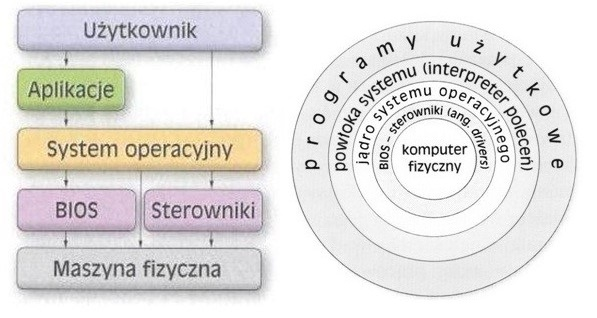
\includegraphics[scale=0.8]{obrazy/warstwowy-model-systemu.jpg}
\caption{Warstwowy model systemu}
\label{rys:warstwowy_model_OS}
\end{figure}

\paragraph{Główne zadania OS}
\begin{itemize}
\item zarządzanie zasobami komputera - systemy operacyjne staruję oraz optymalizują wykorzystanie określonych urządzeń, które wchodzą w skład zestawu komputerowego; specjalne moduły zwane sterownikami, które składają się na system operacyjny udostępniają aplikacjom spójne metody programowania urządzeń (interfejsy), co gwarantuje współdziałanie każdego nowego urządzania z oprogramowaniem (jeżeli producent dostarczy właściwy sterownik)
\item gromadzenie oraz zarządzanie danymi - systemy operacyjne wyposażone są w modułu obsługujące system plików, czyli struktury umieszczone na dyskach, pomagające w logiczny sposób uporządkować dane, grupując je w katalogi i pliki
\item maszyny wirtualne - systemy operacyjne udostępniają aplikacjom tzw. maszyny wirtualne, czyli uproszczone obrazy maszyn, na których pracują aplikacje; system udostępnia aplikacjom szczegóły dna temat komputera oraz rozszerzenia ułatwiające pracę (np. zasoby udostępniane poprzez sieć aplikacje widzą tak, jakby znajdowały się one na dysku lokalnym; aplikacja, która korzysta z takiego zasobu nie obsługuje pracy sieciowej, więc aby umożliwić jej dostęp do zasobu, system operacyjny symuluje, jest zasób ten jest lokalny udostępniając go dla aplikacji)
\item wielozadaniowość - na pojedynczym komputerze funkcjonować może wiele aplikacji w jednym czasie; każda aplikacja otrzymuje swoją maszynę wirtualną i może pracować jakby była pojedynczym programem działającym na maszynie; dzięki takiej właściwości systemów operacyjnych nie ma potrzeby przystosowywania aplikacji, by mogła dzielić się daną maszyną z innymi aplikacjami
\item interakcja z użytkownikiem - rolę tę spełnia najbardziej zewnętrzna warstwa systemu operacyjnego zwana powłoką (ang. shell), która pozwala użytkownikowi uruchamiać aplikacje; w systemach graficznych do powłoki zaliczają się także typowe elementy interfejsu, z których korzysta aplikacja, jak kontrolki czy okna dialogowe
\item komunikowanie się z innymi komputerami - jest to jeden z najistotniejszych elementów systemów operacyjnych; dzięki modułom obsługi sieci można uzyskać dostęp do Internetu, do dysków komputerów stojących w sąsiednim pomieszczeniu czy sieciowych urządzeń peryferyjnych jak drukarki czy skanery
\end{itemize}

\paragraph{Najważniejszymi cechami, które decydują o użyteczności danego systemu operacyjnego są:}
\begin{itemize}
\item prostota instalacji oraz użytkowania systemu
\item współpraca z innymi systemami, czyli możliwość odczytu i zapisu danych na partycjach z innych systemów a także współpraca oraz wymiana danych między komputerami w sieciach lokalnych i Internecie
\item zgodność sprzętowa (instalację na konkretnej maszynie utrudnia czasami brak właściwych sterowników dla określonych urządzeń)
\item wymiana danych, czyli możliwość przeglądania oraz wymiany dokumentów pomiędzy różnymi aplikacjami pracującymi pod kontrolą różnych systemów
\item możliwość pracy sieciowej (wygoda podczas przeglądania zasobów sieciowych, wymiany protokołów, itp.)
\item cena
\item liczba aplikacji, które działają w danym systemie (nawet najlepiej pracujący system będzie niemal bezużyteczny, jeżeli oferta oprogramowania, które współpracuje z tym systemem będzie niewielka)
\item lokalizacja (możliwość komunikacji użytkownika z systemem w ojczystym języku)
\end{itemize}

Schemat z rysunku \ref{rys:warstwowy_model_OS}. przedstawia ogólną budowę systemu operacyjnego. Podstawową częścią OS jest jądro systemu (kernel). Jądro odpowiedzialne jest za pracę systemu i wykonywanie wszystkich jego zadań. 

Jądro poprzez sterowniki i BIOS komunikuje się z elektroniką komputera. Aby użytkownik mógł komunikować się z jądrem, system operacyjny posiada powłokę (Shell lub też interpreter). Powłoka systemowa jest to program pełniący rolę pośrednika pomiędzy całym systemem operacyjnym a użytkownikiem. Powłoki mogą być tekstowe lub graficzne.

\begin{figure}[htbp]
\centering
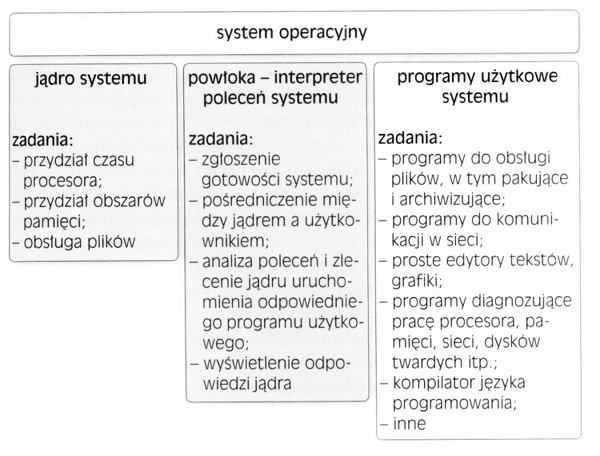
\includegraphics[scale=0.7]{obrazy/zadania-systemu-operacyjnego.png}
\caption{Składniki systemu operacyjnego i ich zadania}
\label{rys:zadania_systemu_operacyjnego}
\end{figure}


\subsubsection{Podział systemów operacyjnych}
\subparagraph{Ze względu na sposób komunikacji systemu z użytkownikiem:}
\begin{itemize}
\item \textbf{systemy tekstowe} - komunikacja przebiega przy pomocy komend wprowadzanych z linii poleceń (DOS, CP/M)
\item \textbf{systemy graficzne} - komunikacja odbywa się przy pomocy graficznych symboli (okienek oraz ikon); obsługa systemu polega na manipulacji przy pomocy myszy bądź klawiatury symbolami odpowiadającym określonym zadaniom (MC Windows, MacOS)
\end{itemize}

\subparagraph{Ze względu na architekturę systemu:}
\begin{itemize}
\item \textbf{monolityczne} - jednozadaniowe systemy posiadające najprostszą strukturę, gdzie w danym czasie może być realizowane tylko jedno zadanie
\item \textbf{warstwowe} - posiadające hierarchiczną strukturę poleceń systemowych; możliwa jest realizacja wielu zadań jednocześnie (np. nadzorowanie procesu drukowania podczas edycji tekstu)
\item \textbf{klient/serwer} - systemy posiadając bardzo rozbudowaną strukturę, nadzorujące podrzędne systemy zainstalowane na komputerach w sieci; systemy te postrzegają aplikacje jako klientów, korzystających z usług serwerów; aplikacja ,,klient'' komunikuje się z serwerem przez jądro systemowe, natomiast każdy serwer działa we własnej, chronionej i wydzielonej przestrzeni adresowej w pamięci operacyjnej, gdzie jest odizolowany od innych zadań; systemy klient/serwer realizują swe zadania na trzy sposoby:
\item wszelkie aplikacje uruchamiane są na serwerze, a wyniki prezentowane u ,,klienta''
\item serwer dostarcza zasobów dla aplikacji, które uruchamiane są po stronie klienta
\item wszelkie komputery współdziałają ze sobą na zasadzie równy z równym (ang. peer to peer), wykorzystując wzajemnie swoje zasoby
\end{itemize}

\subsubsection{Przykłady OS}
\begin{itemize}
\item Windows
\item Linux
\item Unix
\item OS X/ Mac OS X
\item Android
\end{itemize}

\section{Zadania optymalizacji i techniki ich rozwiązywania}

\subsection{Sformułowanie zadania optymalizacji}


Wektor zmiennych decyzyjnych x:
\[x=[x_1, x_2,...x_n]^T,\]
gdzie:\\
n - ilość zmiennych decyzyjnych.
\\\\
Funkcja celu (funkcja kryterialna) f(x):  
\[f(x)~:~R^n \longrightarrow R^1\]
oraz m funkcji ograniczeń $g_i(x)$:
\[g_i(x): R^n \longrightarrow R^1~~dla~i=1,...,m\]

Zadanie optymalizacji polega na znalezieniu wektora zmiennych decyzyjnych 
x, należącego do zbioru rozwiązań dopuszczalnych \textbf{X} w postaci:
\[X = {x|g_i(x) \le 0,~~i=1,...,m}\]
takiego, że dla wszystkich $x \in X$
\[f(\hat{x})<= f(x).\]
Co jest równoznaczne zapisowi:
\[min_{x \in X} f(x) = f(\hat{x}).\]

\subsection{Rodzaje zadań}


\subsubsection{Zadanie programowania liniowego PL} 

\[ max f(x) = c^T x \]
przy ograniczeniach: 
\[A_1 x \le b_1\]
\[A_2 x \ge b_2\]
\[x \ge 0\]
  
\begin{center}
dim x=n, dim c = n
\end{center}
Macierze $A_1, A_2$ odpowiadają za współczynniki w $m_1 i m_2$ ograniczeniach
\\
Wektory $b_1, b_2$ odpowiadają za prawe strony ograniczeń
\\ \\
Przypadki szczególne rozwiązania zadania programowania liniowego
(PL)

\begin{itemize}
\item Istnieje jedno rozwiązanie optymalne zadani PL.
\item Zadanie PL jest zadaniem nieograniczonym – brak rozwiązania.
\item W zadaniu PL zbiór rozwiązań dopuszczalnych jest pusty – brak
rozwiązania.
\item W zadaniu PL wszystkie zmienne lub ich część przyjmuje
\item wartości rzeczywiste.
\item Zadanie PL posiada nieskończoną liczbę rozwiązań.
\end{itemize}
 
\subparagraph{Metody rozwiązywania:}
\begin{itemize}
\item simpleks
\item dwufazowy simpleks
\item dualny simpleks
\end{itemize} 
 
\subsubsection{Zadanie liniowego programowania całkowitoliczbowego PCL}

Zagadnieniem liniowym całkowitoliczbowym nazywamy zadanie optymalizacji
liniowej, w którym wszystkie zmienne lub ich część są liczbami całkowitymi.

\[max_{x \in X} x_0 = c^Tx~~dla~x \in X \subset R^n\]


dla każdego $$1 \le i \le t~~~x_i \in \mathbb{Z}$$

\subparagraph{Metody uproszczone:}
\begin{itemize}
\item Przegląd zupełny zbioru rozwiązań dopuszczalnych X
\item Zaokrąglenie rozwiązania optymalnego zadania PL do zmiennych całkowitych
\end{itemize}

\subparagraph{Metody złożone:}
\begin{itemize}
\item Metoda odcięć Gomory'ego
\item Metoda podziału i ograniczeń
\item Metody przybliżone = metody heurystyczne
\end{itemize}


\subsubsection{Zadanie programowania nieliniowego PN}

$$min_{x \in X} f(x) = f(\hat{x})$$
przy ograniczeniach:
$$X={x|g_i(x)=<0, i=1,...,m|}$$ 
\\
Zadanie programowania nieliniowego polega na znalezieniu wektora zmiennych decyzyjnych $\hat{x}$, należącego do zbiory rozwiązań dopuszczalnych \textbf{X} w postaci: 

takiego, że dla

$$x \in X$$

$$f(\hat{x})=<f(x)$$


\subsubsection{Nieliniowe zadanie optymalizacji statycznej bez ograniczeń}


Funkcja celu f(x):
$$f(x):R^n \longrightarrow R^1$$
\\
Zadanie optymalizacji polega na znalezieniu wektora zmiennych decyzyjnych x, należącego do zbioru rozwiązań dopuszczalnych $R^n$

takiego, że dla każdego $ x \in R^n $


$$ f(\hat{x})\le f(x) $$

Co jest równoznaczne zapisowi:

$$min_{x \in R^n} f(x) = f(\hat{x})$$
\\
\subparagraph{Iteracyjne algorytmy optymalizacji:}
\begin{itemize}
\item Algorytmy optymalizacji w kierunku
\item Algorytmy optymalizacji bez ograniczeń
\item Algorytmy optymalizacji z ograniczeniami
\end{itemize}
Algorytm optymalizacji lokalnej - przemierzanie obszaru rozwiązań dopuszczalnych w poszukiwaniu ekstremum funkcji celu według iteracyjnego schematu.

\subparagraph{Algorytmy bezgradientowe:}
\begin{itemize}
\item Algorytm Nelder’a-Meade’a ( Matlab - funkcja fminsearch)
\item Algorytm Gauss’a-Seidla
\item Algorytm Powella 
\end{itemize}

\subparagraph{Algorytmy gradientowe:}
\begin{itemize}
\item Algorytm największego spadku
\item Zmodyfikowany algorytm Newtona ( Matlab – wersja metody QuasiNewton
- funkcja fminunc)
\item Algorytm Zangwilla
\item Algorytm Fletchera-Reeves’a
\item Algorytm Polaka-Ribiery
\item Algorytm Fletchera-Powella-Davidona
\end{itemize}


\subsubsection{Nieliniowe zadanie optymalizacji statycznej z ograniczeniami}
Znaleźć wektor rozwiązań optymalnych $\hat{x}, taki, że:$

$$f(\hat{x})=min_{x \in X}f(x)$$

gdzie:

$$X={x:g_i(x) \le 0,~~i=1,...,m}$$

$$f:X = R^n \longrightarrow R^1$$

oraz $$g_i:X = R^n \longrightarrow R^1~dla~każdego~i=1,...,m$$

\subparagraph{Ograniczenie aktywne\\\\}

Dla $\hat{x}$ ograniczenie przyjmuje postać:
\[  g_i(\hat{x})=0 \]


$$ g_i(\hat{x}+\tau d) \le 0, dla każdego i \in A(\hat{x})$$

przy czym $\tau \in [0,\sigma]$



\subparagraph{Przypadki:}

\begin{enumerate}

\item \textbf{Jedno ograniczenie aktywne} – rozwiązanie optymalne na brzegu ograniczenia
aktywnego.
\item \textbf{Wszystkie ograniczenia aktywne} - rozwiązanie optymalne na przecięciu ograniczeń
aktywnych.
\item \textbf{Brak ograniczeń aktywnych} – rozwiązanie optymalne wewnątrz obszaru rozwiązań
dopuszczalnych ( rozwiązanie optymalne zadania bez ograniczeń spełnia
ograniczenia problemu.
\end{enumerate}

\section{Systemy dynamiczne, opisy własności}

\paragraph{Układ dynamiczny} - model matematyczny rzeczywistego zjawiska przyrody, którego przyszłe zachowanie(stan,ewolucja) jest wyznaczone jednoznacznie przez stan początkowy i sygnał sterujący. Najczęściej jest opisany pewnym wektorowym równaniem różniczkowym -zwanym równaniem stanu układu. 
\subsection{Podział układów}
\paragraph{Ze względu na charakter sygnałów}
\begin{itemize}
	\item \textbf{Ciągłe }- wszystkie sygnały (wejściowe i wyjściowe) są funkcjami ciągłymi w czasie i mogą
	przybierać dowolna wartość z obszaru swojej zmienności. Układy te opisuje się zwykle równaniami różniczkowymi.
	\item \textbf{Dyskretne} - układ jest dyskretny, jeżeli przynajmniej jeden jego sygnał ma charakter dyskretny,
	tzn. przyjmuje tylko określone wartości dla określonych argumentów. Układy takie opisuje się zwykle równaniami
	różnicowymi.
\end{itemize}
\paragraph{Ze względu na charakter układu}
\begin{itemize}
	\item \textbf{Statyczne} (bezinercyjne) - wyjście w
	danej chwili czasu zależy tylko od wejścia (brak
	stanu nieustalonego). Układy te składają się
	tylko z elementów rozpraszających energie i
	opisuje się je równaniami algebraicznymi.
	\item \textbf{Dynamiczne} - układy, w których wyjście
	nie jest jednoznaczna funkcja wejścia i zależy
	dodatkowo od charakteru procesu
	przejściowego (inercyjności) i stanu układu w
	chwili początkowej. Układy te zawierają
	elementy magazynujące energie. Opisuje się je
	równaniami różniczkowymi lub różnicowymi.
\end{itemize}  
\paragraph{Ze względu na liniowość układu}
\begin{itemize}
	\item \textbf{Liniowe} - można je opisać za pomocą liniowych równań
	algebraicznych, różniczkowych lub różnicowych.
	\textbf{Spełniają one zasadę superpozycji!}
	\item \textbf{Nieliniowe} - zawierające przynajmniej jeden element
	nieliniowy.
\end{itemize}

W praktyce każdy układ fizyczny jest nieliniowy. Model linowy powstaje
	na podstawie przybliżenia zakładającego liniowość fizycznego
	zjawiska i stałość parametrów lub w wyniku linearyzacji wyznaczonej
	nieliniowej charakterystyki. Linearyzacje przeprowadza się zwłaszcza
	wtedy, gdy działanie procesu ogranicza się do niewielkiego obszaru
	wokół pewnego ustalonego punktu pracy.
	
\paragraph{Ze względu na liczbę wejść i wyjść}
\begin{itemize}
\item O jednym wejściu i jednym wyjściu
 \item  O wielu wejściach lub wielu wyjściach
\end{itemize}
\paragraph{Ze względu na  liczbę zmiennych niezależnych}
\begin{itemize}
\item Jednowymiarowe
 \item Wielowymiarowe
\end{itemize}

\paragraph{Ze względu na czasowy charakter parametrów}
\begin{itemize}
\item Stacjonarne – parametry układu nie ulegają zmianie w czasie (lub ich zmiany są pomijalne)
 \item Niestacjonarne – parametry układu ulegają zmianie w czasie
\end{itemize}

\paragraph{Ze względu  na zmienność struktury}
\begin{itemize}
\item O stałej strukturze – takie, które w czasie swojego działania nie zmieniają liczby sygnałów pomiędzy poszczególnymi członami)
 \item O zmiennej strukturze – układy nie spełniające powyższej zasady
\end{itemize}

\paragraph{Ze względu na przestrzenny charakter parametrów}
\begin{itemize}
\item O parametrach skupionych
 \item O parametrach rozłożonych
\end{itemize}

Układ o parametrach rozłożonych – jeśli $n \to \infty $ (czyli jego przestrzeń stanów jest nieskończenie wymiarowa), to układ dynamiczny jest układem o parametrach rozłożonych lub układem nieskończenie wymiarowym. Przeciwieństwem układów o parametrach rozłożonych są układy o parametrach skupionych, dla których $n$ przybiera bardzo duże wartości, ale są to wartości skończone – dlatego układy takie nazywa się też układami \textbf{skończenie wymiarowymi}.	
	
	
	
\subsection{Transmitancja operatorowa układu}
\textbf{Transmitancja operatorowa} (funkcja przejścia, $G(s)$) - stosunek transformaty Laplace`a sygnału wyjściowego do transformaty Laplace`a sygnału wejściowego układu przy zerowych warunkach początkowych.
\begin{equation}
G(s)=\dfrac{Y(s)}{U(s)}
\end{equation}

Transmitancja określa ogólne własności stacjonarnego układu liniowego o jednym wejściu i jednym wyjściu, niezależne od rodzaju wymuszenia. Dla układu wielowymiarowego o $r$ wejściach o $m$ wyjściach można określić $m \times n$ transmitancji wiążących każde wyjście z każdym wejściem.
\subsection{Charakterystyki}
\subsubsection{Czasowa}
{\textbf{Charakterystyka czasowa}} układu liniowego jest jego odpowiedz na określone
wymuszenie przy założeniu zerowych warunków początkowych. Sygnałem
wejściowym może być impuls Diraca $ \delta(t) $, skok jednostkowy 1(t) (funkcja
Heaviside’a) lub sygnał narastający liniowo (rampa).\\

Należy zaznaczyć, że zarówno impuls Diraca, jak i skok jednostkowy są sygnałami niemożliwymi do generacji z uwagi na skończoną szybkość zmian
wartości sygnałów (na przykład skończoną prędkość przestawiania zaworu
przez siłownik) lub niebezpieczeństwo wywołania dynamicznego wejścia
obiektu rzeczywistego w zakres nieliniowości.
		
\subsubsection{Skokowa}
\paragraph{Charakterystyką skokową} (odpowiedzią skokową) $h(t)$ układu liniowego jest
jego odpowiedz na wymuszenie skokiem jednostkowym $u(t) = 1(t)$ przy
zerowych warunkach początkowych. Jest ona bardzo ważnym elementem teorii
sterowania, ponieważ opisuje właściwości dynamiki układu w zależności
jedynie od jego parametrów i pojedynczej wartości opisującej skok (amplitudy).\\\\
Charakterystyka skokowa umożliwia proste wyznaczenie współczynnika
		wzmocnienia obiektu statycznego, równego stosunkowi wartości ustalonej
		odpowiedzi skokowej do wartości sygnału wejściowego.
		
\subsubsection{Impulsowa}
\paragraph{Charakterystyką impulsową} (odpowiedzią impulsową) $g(t)$ układu liniowego
jest jego odpowiedz na wymuszenie impulsem Diraca $u(t)=\delta(t) $ przy zerowych
warunkach początkowych. Podobnie jak charakterystyka skokowa opisuje
również właściwości dynamiki układu w zależności od jego parametrów.
Charakterystyka impulsowa umożliwia w prosty sposób określić, czy obiekt jest
astatyczny – w tym przypadku wartość $g(t)$ w stanie ustalonym jest niezerowa.

\subsubsection{Charakterystyka amplitudo-fazowa}
\paragraph{Charakterystyką amplitudowo-fazową (wykresem Nyquista)} nazywa się wykres
transmitancji widmowej na płaszczyźnie zmiennej zespolonej, przy czym na osi
rzędnych (osi liczb rzeczywistych) odłożona jest wartość $P(\omega)$, a na osi
odciętych (osi liczb urojonych) wartość $Q(\omega)$. Przykład takiego wykresu został ukazany na rys. \ref{rys:dynamiczne_wykres_nyquista}.
\begin{figure}[htbp]
	\centering
	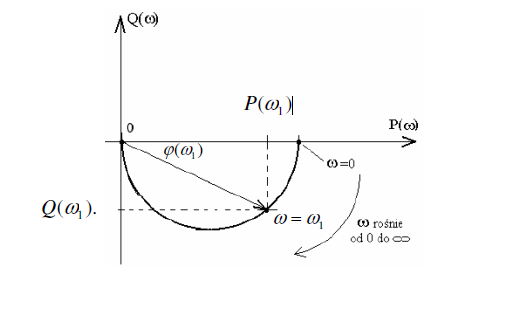
\includegraphics[scale=0.7]{obrazy/dynamiczne/nyquist.png}
	\caption{Przykład wykresu Nyquista}
	\label{rys:dynamiczne_wykres_nyquista}
\end{figure}

\subsection{Człony dynamiczne}
Rozdział 3. (dokładnie 9 stron) z książki prof. Greblickiego.

\subsection{Stabilność}
Stabilność jest jest jedną z najważniejszych własności, której wymaga się od systemu dynamicznego.

\subsubsection{Twierdzenia i definicje}
\paragraph{Definicja stabilności\\} Jeśli przy zerowym pobudzeniu i każdym warunku początkowym:
\begin{center}
	$ \lim_{t\to\infty}y(t)=0 $
\end{center}
to system nazywamy stabilnym.
System jest stabilny wtedy i tylko wtedy, gdy wszystkie bieguny jego transmitancji leżą w lewej półpłaszczyźnie płaszczyzny liczb zespolonych.
\paragraph{Granica stabilności\\} System znajduje się na granicy stabilności wtedy i tylko wtedy:
\begin{center}
	$Res_{1}\le0,Res_{2}\le0,...,Re s_{m}\le0, $
\end{center}
przy czym bieguny transmitancji, dla których zachodzą równości są co najwyżej jednokrotne.

\subsubsection{Kryteria stabilności}
Aby stwierdzić czy system o transmitancji:
$$K(s)=\frac{L(s)}{M(s)} $$
jest stabilny, wystarczy rozwiązać jego równanie charakterystyczne $M(s)=0$, a następnie sprawdzić, czy wyznaczone w ten sposób pierwiastki mają ujemne części rzeczywiste 

Rozwiązanie równania jest możliwe tylko dla $m \le 4 $ tzn. tylko wtedy można znaleźć jego pierwiastki przy użyciu takich działań jak dodawanie, odejmowanie, mnożenie i dzielenie oraz pierwiastkowanie. Równań wyższych stopni, poza szczególymi przypadkami, rozwiązać nie można.
$$M(s)=a_{m}s^{m}+a_{m-1}s^{m-1}+...+a_{1}s+a_{0} $$


\paragraph{Twierdzenie o znaku współczynników\\}
Jest to warunek konieczny.

Niech $ a_{m}>0 $. Jeśli system jest stabilny to:

	$$ a_{0}>0,a_{1}>0,...,a_{m-1}>0. $$

\paragraph{Kryterium Routha-Hurwitza\\}
Jest to warunek wystarczający. Jeśli:
$$\Delta_{1}\neq 0,~~\Delta_{2}\neq 0,~~...,~~\Delta{m}\neq 0 $$
to żaden z pierwiastków wielomianu M(s)nie leży na osi $j\omega $.
Z twierdzenia wynika oczywisty wniosek, że jeśli wszystkie $ \Delta$ są większe od zera to system jest stabilny.

\paragraph{Kryterium odpowiedzi skokowej\\}

Układ zamknięty w odpowiedzi na skok jednostkowy powinien osiągać stan ustalony w czasie dążącym do nieskończoności.

\paragraph{Kryterium Hurwitza\\}
Niech $ a_{m}>0$. System jest stabilny wtedy i tylko wtedy gdy:
\begin{center}
	$$\Delta_{1}>0,~~\Delta_{2}>0,~~...,~~\Delta{m}>0.$$
\end{center}
Warunek konieczny i wystarczający.
\paragraph{Kryterium Michajłowa\\}
Niech $ a_{m}>0$. System jest stabilny wtedy i tylko wtedy, gdy:
	\begin{center}
	$ M(j\omega)\neq 0$ dla wszystkich $\omega \in [0,\inf) $
	\end{center}
oraz
	$$\Delta arg M(j\omega)= m\frac{\pi}{2}  $$

\begin{figure}[htbp]
	\centering
	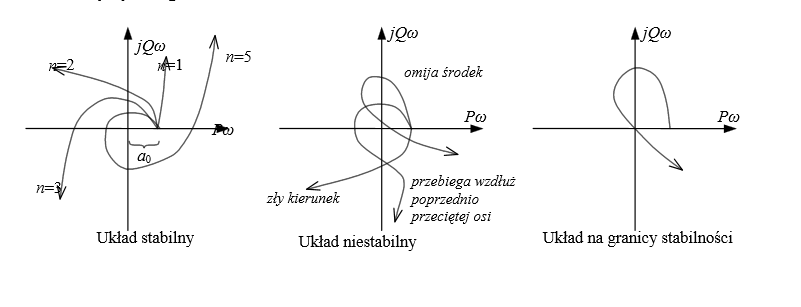
\includegraphics[scale=0.7]{obrazy/dynamiczne/Michajlow_przyklad.png}
	\caption{Przykład zastosowania kryterium Michajłowa do określenia stabilności systemu}
	\label{rys:dynamiczne_kryterium_michajlowa}
\end{figure}
Układ automatycznej regulacji jest stabilny, gdy zmiana argumentu funkcji N(j$\omega$) przy zmianie pulsacji $\omega$
od zera do +$\inf$ wynosi n$\frac{\pi}{2}$, gdzie n oznacza stopień równania charakterystycznego. Przykład zastosowania kryterium Michajłowa do określenia stabilności systemów został przedstawiony na rys. \ref{rys:dynamiczne_kryterium_michajlowa}.

\paragraph{Kryterium Nyquista\\}
Układ zamknięty jest stabilny, jeżeli logarytmiczna charakterystyka amplitudowa układu otwartego posiada wartość ujemną dla pulsacji odpowiadającej przesunięciu fazowemu - $\pi$. Przykład zastosowania kryterium Nyquista do określenia stabilności systemu został ukazany na rys. \ref{rys:dynamiczne_przyklad_nyquist}.
\begin{figure}[htbp]
	\centering
	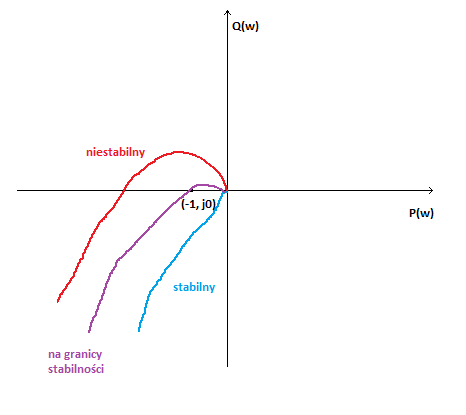
\includegraphics[scale=0.7]{obrazy/dynamiczne/Przyklad_nyquist.png}
	\caption{Przykład zastosowania kryterium Nyquista do określenia stabilności systemu}
	\label{rys:dynamiczne_przyklad_nyquist}
\end{figure}
\\
Gdyby ktoś potrzebował większego przypomnienia z kryteriów: 
\href{http://home.agh.edu.pl/~pautom/pliki/wyklady/przykladowe/08.pdf}{\url{http://home.agh.edu.pl/~pautom/pliki/wyklady/przykladowe/08.pdf}}
+ warto przypomnieć sobie rozwiązywanie równań różniczkowych.


\section{Programowanie w systemie operacyjnym Unix}

%\subsection{Interpreter komend Bourne shell, podstawowe mechanizmy, pisanie skryptów, rozszerzenia POSIX }

\subsection{Programowanie w języku powłoki}

\paragraph{Powłoka} (ang. shell) jest programem umożliwiającym pracę z systemem   UNIX. Jej nazwa wywodzi się z graficznej prezentacji systemu, w której jądro i procesy obsługi wejścia i wyjścia są otoczone właśnie przez powłokę. Jej funkcją jest odseparowanie użytkownika od bezpośredniego dostępu do jądra systemu i umożliwienie   łatwej i wszechstronnej pracy. Podstawowym zadaniem powłoki jest przyjmowanie     poleceń użytkownika i uruchamianie stosownych programów. Do dalszych funkcji powłoki należy konstruowanie parametrów dla poleceń oraz zarządzanie sposobem wykonywania programów procesów. Następnym, bardziej skomplikowanym krokiem jest tworzenie   funkcji i procedur powłoki(skryptów) pozwalających   na łączenie wielu   poleceń  w   jedno,umożliwiając pisanie całych programów dla powłoki.
\subsubsection{Powłoki UNIX}
\begin{itemize}
\item \textbf{Bourne shell (sh)}
	\begin{itemize}
	\item nie umożliwia ona operowania na liczbach całkowitych bez tworzenia nowego procesu
	\item plikiem wykonywalnym powłoki na większości systemów Unix jest /bin/sh
	\item  podstawowa powłoka w każdym systemie typu Unix
	\end{itemize}
\item \textbf{Bash}
	\begin{itemize}
	\item umożliwia wykonanie obliczeń za pomocą wyrażeń w podwójnych nawiasach ((...)) oraz składni \$[...]
	\end{itemize}
\item \textbf{Korn shell (ksh)}
	\begin{itemize}
	\item kompatybilna wstecz z sh
	\item zawiera wiele elementów z csh, np. historię komend
	\end{itemize}
\item \textbf{C shell (csh)}
	\begin{itemize}
	\item o składni języka C
	\item pochodzi od sh
	\item ulepszenia: aliasy i historia komend
	\item jej następcą jest tcsh
	\item rzadko wykorzystywana
	\end{itemize}
\end{itemize}


\subsubsection{Polecenia powłoki}
Wydanie polecenia w powłoce wiąże się z podaniem ciągu znaków. Składa się z następujących elementów:
\begin{center}\textbf{<nazwa polecenia> -<opcje> <parametry>}\end{center}
Nazwą polecenia jest nazwa jakiegokolwiek programu, funkcji powłoki lub funkcji   wewnętrznej powłoki. Opcje to najczęściej zestaw pojedynczych liter określających     sposób wykonania programu. Parametry to informacje czego dotyczy wykonanie.

\subsection{Podstawowe mechanizmy}
\subsubsection{Globbing}
Mechanizm polegający na dopasowywaniu.
$*$ $?$ $[a-z A-Z_]$ do nazw plików.

\subsubsection{Procesy i podprocesy\\}
Wykonywanie programów powoduje utworzenie oddzielnego procesu, który jest podprocesem interpretera poleceń. Proces ma dostęp do standardowych urządzeń wejść i wyjść: stdin, stout, stderr, oraz środowiska, które jest zestawem zmiennych z przypisanymi wartościami.

\subsubsection{Potoki}
Potoki to równoległe uruchomienie dwóch lub więcej poleceń z szeregowym połączeniem ich wejść i wyjść.

\subsubsection{Prawa dostępu}

Mechanizm w systemach uniksowych, mający na celu umożliwić określenie uprawnień odczytu, edycji i uruchamiania dla poszczególnych użytkowników. Ma on na celu zapewnienie bezpieczeństwa, stabilności i kontroli prywatności w systemach wielodostępnych.
Prawa dostępu przydzielane są dla kategorii: user,    group,  other.
Dla każdej z tych kategorii możliwe są trzy prawa dostępu, opisane literowo (rwx) lub liczbowo trzema bitami: read, write, execute. 


\subsubsection{Pisanie skryptów}

Skrypty to pliki zawierające zestaw poleceń interpretera. Skrypt można uruchomić jawnie wywołując interpreter poleceń podając nazwę skryptu jako argument.


\subsubsection{Rozszerzenia POSIX}


\paragraph{POSIX (ang. Portable Operating System Interface for Unix)} – przenośny interfejs dla systemu operacyjnego Unix. Jest zbiorem norm, mających zestandaryzować cechy i interfejsy, które powinien mieć i zapewniać system UNIX. 
Standaryzuje między innymi: operatory arytmetyczne, lokalizacje, klasy mechanizmu globbingu, polecenia zagnieżdżone.


\subsection{Wyrażenia regularne: sed, awk, grep} 

\subsubsection{sed}

sed (od ang. stream editor) – edytor strumieniowy, służy do przetwarzania tekstu.
Edytor sed
wczytuje   bieżący   wiersz   pliku   do   wewnętrznego   bufora   celem
manipulowania   tekstem.   Wynik   jest   wysyłany   na   standardowe   wyjście.
Oryginalny plik nie jest nigdy zmieniany. 
\\
Składnia uruchamiania sed: sed 
opcje 'polecenie' nazwa\_pliku
Wybrane polecenia: wyświetlenie linii, opuszczenie pustych linii, zakończ, skasowanie linie, zapisanie linii do pliku.

\subsubsection{awk}

Uniwersalny filtr programowalny. 
\begin{itemize}
	\item Czyta wiersz z wejścia, dzieli na pola (słowa) dostępne jako: \$1, \$2, ...
	\item Wykonuje program składający się z par warunek - akcja.
	\item Par warunek-akcja może być wiele i w każdej może brakować warunku.
	(domyślnie: prawda) albo akcji (domyślnie: wyświetlenie wiersza.
	\item Zmienne zachowują wartości pomiędzy wierszami.
\end{itemize} 
Jego główną funkcją jest wyszukiwanie i przetwarzanie wzorców w plikach lub strumieniach danych.

\subsubsection{grep}

Program który służy do wyszukiwania w tekście i wyodrębniania linii zawierających ciąg znaków pasujący do podanego wyrażenia regularnego.\\
Użycie: \$ grep opcje wzorzec plik/pliki\\\\
Przykładowe opcje: \\
-w – wyszukuje tylko całe słowa;\\
-x – wyszukuje tylko całe linie;\\
-c –  wyświetla liczbę znalezionych linii.


\subsection{Funkcje I/O niskiego poziomu, deskryptory, przegląd bibliotek systemu UNIX}

\subsubsection{Funkcje I/O niskiego poziomu}
Funkcje open, read, write, zwane wbudowanym systemem we/wy niskiego poziomu, są głównym systemem operacji na plikach i urządzeniach w Unixie.
Odwołują się do otwartych plików przez numery deskryptorów.

\subsubsection{Deskryptory}
To małe liczby przyporządkowane kolejno otwieranym plikom. Programy uzyskują najniższy wolny deskryptor. Jeśli inny proces otworzy ten sam plik otrzyma własny (inny lub ten sam) numer deskryptora. Operacja odczytu może przebiegać jednocześnie dla wielu procesów. Jeśli procesy otworzą jednocześnie plik do zapisu, nadpiszą się wzajemnie, konieczna jest synchronizacja w postaci blokad. 

\subsubsection{Przegląd bibliotek systemu UNIX}
\begin{itemize}
	\item \textbf{stdio} - 	działa podobnie jak operacje I/O niskiego poziomu.
	\item \textbf{string} 
	\item \textbf{crypt} 
	\item \textbf{ndbm} - tworzenie własnych baz danych dla dużej ilości danych i dużej przenoszalności.
\end{itemize}

\subsection{Programowanie procesów: tworzenie, atrybuty, dziedziczenie atrybutów, współdzielenie zasobów. Sygnały, obsługa sygnałów. Komunikacja przez potoki}

\subsubsection{Programowanie procesów}
Procesy mają: kod programu w pamięci, środowisko (zmienne i wartości), zestaw dalszych informacji np. tablicę otwartych plików, priorytet. \\
\\
Tworzenie procesów poprzez klonowanie istniejącego procesu funkcją fork() (procesy potomek i rodzic). Podproces dziedziczy lub współdzieli pewne atrybuty i zasoby procesu nadrzędego. Proces kończy pracę normalnie (funkcja exit() lub koniec main()) lub anormlanie (synał lub funkcja abort()).\\ 
\\
Przykładowe atrybuty procesu:  PID, PPID, UID, terminal, blokady, maska sygnałów, ograniczenia zasobów.

\subsubsection{Sygnały, obsługa sygnałów.}

Sygnały są mechanizmem asynchronicznego powiadamiania procesów o zdarzeniach. 

Generuje je:
\begin{itemize}
	\item błędy i wyjątki sprzętowe
	\item pewne klawisze terminala
	\item funkcja kill
	\item mechanizmy softwarowe
\end{itemize}

Reakcja procesu możliwa: ignorowanie, wywołanie funkcji, śmierć procesu.\\
\\
Tradycyjna obsługa procesów: zadeklarowanie innej niż domyślna obsługi sygnału ma charakter jednorazowy (zadziała inaczej tylko raz.



\subsection{Komunikacja międzyprocesowa}  

\subsubsection{Komunikacja przez potoki}
\paragraph{Potok (ang. pipe)} to narzędzie szeregowej, jednokierunkowej komunikacji o własnościach:
\begin{itemize}
	\item operacje odczytu i zapisu na potoku jak na zwykłym pliku,
	\item dostępne jako dwa lub jeden deskryptor pliku (oddzielne dla końca zapisu i odczytu),
	\item ma ograniczoną pojemność,
	\item jeśli pusty lub przepełniony - proces obsługi wisi i kontynuuje gdy to możliwe.	
\end{itemize}


\subsubsection{Komunikacja przez gniazdka}
%Gniazdka do deskryptory plików umożliwiające dwukierunkową komunikację w ramach jednego systemu lub przez sieć komputerową. Do korzystania z gniazdek potrzebne jest tworzenie struktury adresowej.Gniazda posiadają również port. Mogą działać jako klient serwer albo broadcast (do wszystkich w sieci).

\paragraph{Gniazdo (ang. socket)} jest mechanizmem komunikacyjnym, który pozwala na implementację systemów klient-serwer albo na lokalnym komputerze, albo w sieciach. Usługi Uniksa, takie jak drukowanie, oraz narzędzia sieciowe, takie jak rlogini ftp, zwykle komunikują się za pomocą gniazd.
Są tworzone i używane w odmienny sposób niż potoki, ponieważ istnieje w nich wyraźne rozróżnienie pomiędzy serwerem i klientem
Mechanizm gniazd w naturalny sposób wspiera implementacje z pojedynczym serwerem i wieloma klientami.
Po stworzeniu gniazda poprzez funkcję systemową \emph{socket} żaden inny proces na razie nie ma do niego dostępu.

Gniazda charakteryzują się trzema atrybutami: domeną, typem i protokołem. Posiadają również adres, który jest używany jako ich nazwa.

\subsubsection{Kolejki komunikatów POSIX}
Mają własności: 
\begin{itemize}
	\item Dwukierunkowe narzędzie komunikacji w jednym z trybów (O\_RDONLY, O\_WRONLY, O\_RDWR).
	\item Stały rozmiar komunikatu.
	\item Nie przekazują komunikatu jako strumień bajtów, ale jako całe jednostki.
	\item Komunikaty posiadają priorytety.
\end{itemize}

\subsubsection{Semafory}
\paragraph{Semafor} jest zmienną kontrolującą przydział danego zasobu. Semafor wykonuje dwie operacje:
\begin{itemize}
\item P - zajęcie zasobu sygnalizowanie zmniejszeniem wartości zmiennej o 1,
\item V - zwolnienie zasobu, zwiększenie zmiennej o 1.
\end{itemize}
Istnieją semafory system V IPC oraz POSIX, choć te pierwsze są kłopotliwe w użyciu.

\section{Komputer, architektura i oprogramowanie}
\paragraph{Komputer} [ang. < łac. computare 'rozważać', 'obliczyć'], elektroniczna maszyna cyfrowa, urządzenie elektroniczne przeznaczone do przetwarzania informacji (danych) przedstawionych w postaci cyfrowej, sterowane programem zapisanym w pamięci.
Pojęcie komputera obejmuje obecnie zarówno komputery zaprogramowane na stałe, używane jako automaty sterujące, np. w urządzeniach gospodarstwa domowego, jak i komputery uniwersalne, dające się dowolnie zaprogramować.

\subsection{Architektury} 
 
\subsubsection{Model von Neumanna a model współczesnego komputera} 
John von Neumann opublikował w 1945 r. propozycję opracowania nowego komputera. Zasadniczą nowością była
koncepcja przechowywania programu w pamięci. Komputer miał składać się z czterech bloków funkcjonalnych:
\begin{itemize}
\item pamięci przechowującej program do wykonania i dane dla niego,
\item jednostki arytmetyczno-logicznej zawierającej rejestry AC (ang. ACcumulator), MQ (ang. Multiplier-Quotier), MBR
(ang. Memory Buffer Register),
\item jednostki sterującej zawierającej licznik programu PC (ang. Program Counter), rejestr adresowy MAR (ang. Memory
Address Register) i pomocnicze rejestry IBR (ang. Instruction Buffer Registers), IR (ang. Instruction Registers),
\item urządzeń wejścia-wyjścia.
\end{itemize}

\subparagraph{Składniki współczesnego komputera:}
\begin{itemize}
\item (mikro)procesor, zawierający co najmniej jedną jednostkę arytmetyczno-logiczną, jednostkę sterująca i rejestry,
\item pamięć operacyjna;
\item urządzenia wejścia-wyjścia (klawiatura, mysz, karta graficzna, pamięci dyskowe itp.),
\item układ bezpośredniego dostępu do pamięci (ang. DMA – Direct Memory Access),
\item układ przerwań.
\end{itemize}
Urządzenia wejścia-wyjścia same też mogą być skomplikowanymi układami mikroprocesorowymi i zawierać w swoim
wnętrzu mikroprocesor, pamięć operacyjną, układy wejścia-wyjścia itd. Układ DMA jest specjalizowanym procesorem odciążającym procesor główny przy operacjach przesyłania dużych bloków danych między pamięcią operacyjną a układami wejścia-wyjścia. Komunikacja pomiędzy poszczególnymi składnikami odbywa się za pomocą szyn (zwanych też magistralami): danych, adresowych, sygnałów sterujących.


\subsubsection{Architektury typu Princeton i Harward}


Architektura typu Princeton posiada wspólną hierarchię pamięci programu i danych, jak opisano to w modelu von
Neumanna. Architektura typu Harward polega na rozdzieleniu pamięci programu od pamięci danych. Stosowana
jest dla zwiększenia wydajności w pamięciach podręcznych oraz w systemach wbudowanych (np. sterownikach
urządzeń AGD, gdzie kod programu nie zmienia się przez całe życie urządzenia lub zmienia się rzadko).

\subsection{Opis składowych komputera}

\subsubsection{Pamięć operacyjna}

\subparagraph{Pamięć operacyjna (ang. internal memory, primary storage)} – pamięć komputerowa adresowana i dostępna bezpośrednio przez procesor, a nie za pośrednictwem urządzeń wejścia-wyjścia. W pamięci tej mogą być umieszczane rozkazy procesora (program) dostępne bezpośrednio dla jego jednostek wykonawczych.

\subsubsection{Urządzenia wejścia-wyjścia} 

\subparagraph{Urządzenie wejścia-wyjścia} służy do komunikacji systemu komputerowego z jego użytkownikiem lub innym systemem przetwarzania danych. Urządzenie wejścia-wyjścia służy często do zamiany wielkości fizycznych na dane przetwarzane przez system lub odwrotnie. Np. mysz komputerowa przetwarza ruch ręki, odbiornik GPS aktualne położenie geograficzne, a monitor komputera przetwarza dane komputerowe na obraz.

\subsubsection{DMA - Direct Memory Access}

\subparagraph{DMA} jest to technika, która umożliwia urządzeniom I/O wysłanie oraz odbieranie danych bezpośrednio do lub z pamięci operacyjnej, pomijając CPU w celu przyspieszenia tych operacji oraz odciążenia procesora, który uczestniczy w procesie w niewielkim stopniu. Ma on za zadanie odpowiednio programować kontroler DMA który zajmuje się transferem danych. 

\subsubsection{System przerwań}

\subparagraph{Przerwanie} to sygnał powodujący zmianę przepływu sterowania, niezależnie od aktualnie wykonywanego programu. Pojawienie się przerwania powoduje wstrzymanie aktualnie wykonywanego programu i wykonanie przez procesor kodu procedury obsługi przerwania (ang. interrupt handler). Procedura ta wykonuje czynności związane z obsługą przerwania i na końcu wydaje instrukcję powrotu z przerwania, która powoduje powrót do programu realizowanego przed przerwaniem.
\begin{itemize}
\item Przerwania sprzętowe (maskowalne, niemaskowalne)
\item Przerwania programowe
\item Praca krokowa
\item Wyjątki
\item Tablica przerwań
\end{itemize}

\subsection{Oprogramowanie}

\paragraph{Oprogramowanie} (ang. software) – całość informacji w postaci zestawu instrukcji, zaimplementowanych interfejsów i zintegrowanych danych przeznaczonych dla komputera do realizacji wyznaczonych celów. Celem oprogramowania jest przetwarzanie danych w określonym przez twórcę zakresie.


\paragraph{Rodzaje oprogramowania}

\begin{itemize}
\item oprogramowanie systemowe - realizujące funkcje konieczne dla działania systemu
\item oprogramowanie do tworzenia oprogramowania
\item biblioteki programistyczne 
\item oprogramowanie użytkowe
\end{itemize}
%\part{Zagadnienia kierunkowe}
\bigskip
\section{Programowanie strukturalne i obiektowe}

\subsubsection{Programowanie strukturalne}
Jest to ,,podparadygmat'' programowania proceduralnego. Opiera się na tworzeniu programów z kilku dobrze zdefiniowanych funkcji takich jak instrukcja warunkowa if-then-else i pętle, za to bez skoków (go to). Proponowane jest używanie tylko trzech struktur sterujących:
\begin{itemize}
\item \textbf{Sekwencja lub konkatencja} – wykonywanie instrukcji w określonej kolejności.
\item \textbf{Wybór} – wykonywanie jednej z kilu instrukcji zależnie od stanu programu. Przykładem jest if-then-else i switch/case.
\item \textbf{Iteracja} - przetwarzanie instrukcji tak długo, jak długo spełniony(lub niespełniony) jest dany warunek. Np. while, for.
Te struktury stosuje się do ,,małych'' bloków programu złożonych z elementarnych instrukcji tj. podstawień, wywołań procedur/funkcji, instrukcji IO itd... Duże bloki powinny być rozbite na mniejsze (funkcje, procedury) tak aby rozumieć poszczególne fragmenty bez rozumienia całości. Podział ten ma również wpływ na jakość kodu, ponieważ procedura/funkcja może być używana wielokrotnie bez niepotrzebnego powielania kodu.
\end{itemize}
\medskip 

\subsubsection{Programowanie obiektowe}
W programowaniu obiektowym program to zbiór porozumiewających się ze sobą obiektów, czyli jednostek zawierających określone dane i umiejących wykonywać na nich określone operacje. Najważniejsze są tu dwie cechy: po pierwsze, powiązanie danych (czyli stanu) z operacjami na nich (czyli poleceniami) w całość, stanowiącą odrębną jednostkę — obiekt; Programowanie obiektowe ułatwia, pisanie, konserwację, testowanie i wielokrotne użycie programów lub ich fragmentów.
\medskip 

Podstawowe założenia paradygmatu obiektowego:
\begin{itemize}
\item \textbf{Abstrakcja} – każdy obiekt w systemie służy jako model abstrakcyjnego „wykonawcy” który może wykonywać pracę (metody), opisywać swój stan, zmieniać swój stan oraz komunikować się z innymi obiektami bez ujawniania jego implementacji.
\item \textbf{Hermetyzacja} – ukrywanie implementacji, enkapsulacja. Zapewnia, że obiekt nie może zmienić statu wewnętrznego innych obiektów w nieoczekiwany sposób. Każdy obiekt prezentuje innym obiektom swój interfejs który określa dopuszczlne metody współpracy.
\item \textbf{Polimorfizm} – wielopostaciowość, referencje mogą dotyczyć obiektów różnego typu. Wywołanie metody dla referencji spowoduje zachowanie odpowiednie dla typu obiektu danej referencji. Jeśli dzieje się to w trakcie wykonywania programu to nazywa się to wiązaniem dynamicznym.
\item \textbf{Dziedziczenie} – porządkuje i wspomaga polimorfizm. Umożliwia definiowanie i tworzenia specjalizowanych obiektów na podstawie bardziej ogólnych (od ogółu do szczegółu). Dzięki temu nie powiela się kodu oraz można redefiniować szczególne parametry bez redefiniowania parametrów ogólnych.
\end{itemize}
\medskip 

Języki wspierające programowanie obiektowe m.in.: C\#, Java, C++, JavaScript, Objective-C
\medskip 

Źródło : materiały PW


\section{Fala elektromagnetyczna: typy, parametry, właściwości}
\subsection{Pojęcia}
\paragraph{Pole elektryczne} – każdy ładunek wytwarza w przestrzeni wokół siebie pole elektryczne, siła elektrostatyczna działająca na dowolny ładunek jest wywołana polem elektrycznym, wytworzonym przez inne ładunki w miejscu w którym znajduje się rozważany ładunek.

\paragraph{Pole magnetyczne} – wytwarzany przez magnes, jest to pole wektorowe tak jak w przypadku pola elektrycznego. W elektromagnesie pole magnetyczne wytwarzane jest za pomocą przepływu prądu przez cewkę nawiniętą na metalowy rdzeń z żelaza. O sile pola decyduje wartość natężenia prądu. Magnesy trwałe zawierają cząstki elementarne (elektrony) które wytwarzają własne pole magnetyczne. W niektórych materiałach pola magnetyczne elektronów sumują się wytwarzając wokół nich wypadkowe pole magnetyczne.

\paragraph{Fala elektromagnetyczna} – jest to rozchodząca się z prędkością c fala pola elektrycznego i magnetycznego. Fale elektromagnetyczne można podzielić na:
\begin{itemize}
\item Fale stojące (punkty o jednakowej fazie nie przemieszczają się) np. wnęka rezonansowa
\item Bieżące (punkty o jednakowej fazie poruszają się) – rozchodzące się wzdłuż linii przesyłowej lub wolnej przestrzeni
\end{itemize}

\begin{figure}[htbp]
\centering
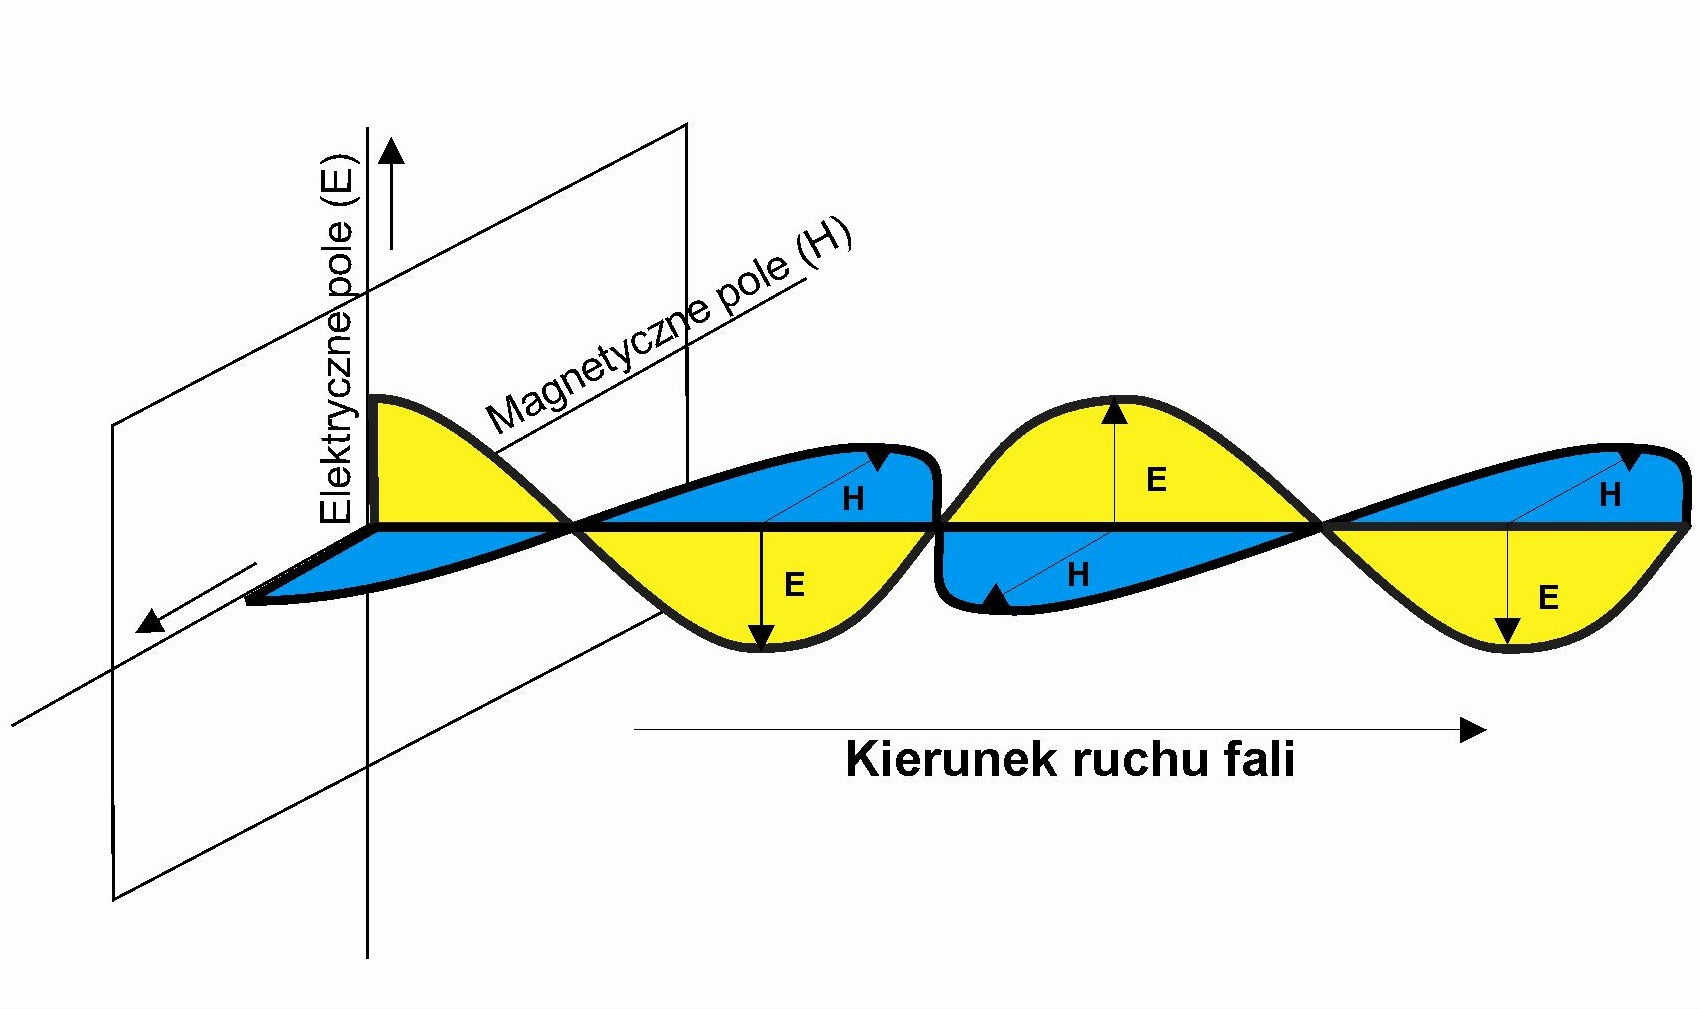
\includegraphics[scale=0.25]{obrazy/fala.jpg}
\caption{Fala elektromagnetyczna}
\label{rys:fala_wektory}
\end{figure}

\subsection{Parametry i właściwości}
\paragraph{Cechy fali EM}
\begin{itemize}
\item Wektory $\overrightarrow{E}$ i $\overrightarrow{B}$ są zawsze prostopadłe do kierunku rozchodzenia się fali. Zatem fale elektromagnetyczna jest falą poprzeczną.
\item Iloczyn wektorowy $\overrightarrow{E} \times \overrightarrow{B}$ zawsze wyznacza kierunek rozchodzenia się fali.
\item Natężenie pola elektrycznego i indukcja pola magnetycznego zmieniają się zawsze sinusoidalnie. Wektory pól zmieniają się z taką samą częstością a ich oscylacje są zgodne w fazie.
\end{itemize}

Rozważając powyższe cechy, przyjmując, że fala rozchodzi się w dodatnim kierunku osi OX. Wektor natężenia pola elektrycznego wykonuje oscylacje równoległe do osi OY a wektor indukcji równolegle do osi OZ (w prawoskrętnym układzie współrzędnych). Można zapisać następujące równania:

\begin{equation}
E(x,t) = E_m \cdot \sin (kx - \omega t) - składowa~elektryczna,
\end{equation}
\begin{equation}
B(x,t) = B_m \cdot \sin (kx - \omega t) - składowa~magnetyczna,
\end{equation}
gdzie:\\
$E_m$ i $B_m$ - amplitudy fali pola elektrycznego i magnetycznego,\\
$\omega$ - częstotliwość kątowa wyrażona przez wektor falowy ($\omega = ck$),\\
$k$ - stała propagacji ($k = 2\pi /\lambda$),\\
$\lambda$ - długość fali ($\lambda=cT$),\\
$T$ - okres drgań.\\

Prędkość fali elektromagnetycznej:
\begin{equation}
c=\dfrac{\omega}{k} = \dfrac{1}{\sqrt{\mu _0 \varepsilon _0}} = 3.0 \cdot 10^8 \dfrac{m}{s},
\end{equation}
gdzie:\\
$\mu _0$ - przenikalność magnetyczna próżni ($4\pi \cdot 10^{-7}~H/m$),\\
$\varepsilon _0$ - przenikalność elektryczna próżni ($8.854 \cdot 10^{-2}~F/m$).\\

\paragraph{Energia fali elektromagnetycznej} – energia pojedynczego kwantu jest zależna tylko od częstotliwości fali f i wynosi:

\begin{equation}
E = \hbar f,
\end{equation}
gdzie:\\
$\hbar$ - stała Plancka ($6.626 \cdot 10^{-34}~J \cdot s$). 

\paragraph{Wektor Poyntinga} – strumień energii przenoszonej przez falę elektromagnetyczną w każdym punkcie przestrzeni określa wektor Poyntinga zdefiniowany, jako:

\begin{equation}
\overrightarrow{S} = \dfrac{1}{\mu _0} \overrightarrow{E} \times \overrightarrow{B}.
\end{equation}

\paragraph{Pęd i ciśnienie fali elektromagnetycznej} – biegnąca fala elektromagnetyczna niesie ze sobą pęd równy:
\begin{equation}
\overrightarrow{p} = \dfrac{W}{c} \hat{k},
\end{equation}
gdzie: \\
$W$ - energia niesiona przez falę,\\
$c$ - prędkość światła,\\
$\hat{k}$ - wektor jednostkowy w kierunku rozchodzenia się fali.

\begin{figure}[htbp]
\centering
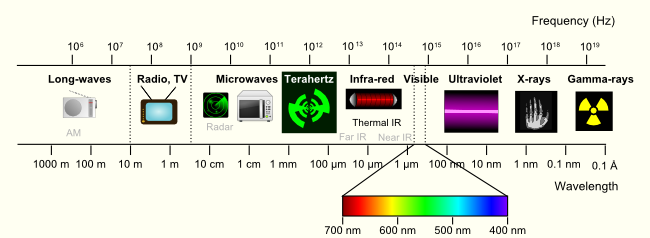
\includegraphics[width=\linewidth]{obrazy/spectrum.png}
\caption{Widmo promieniowania elektromagnetycznego}
\label{rys:widmo}
\end{figure}

\section{Tranzystory bipolarne i unipolarne: budowa, właściwości i zastosowania}

\subsection{Tranzystory bipolarne}  
\paragraph{Tranzystor bipolarny} – półprzewodnikowy element elektroniczny o trzech elektrodach. Jest to najważniejszy przykład elementu aktywnego, czyli urządzenia, które może wytwarzać na wyjściu sygnał o mocy większej niż moc sygnału wejściowego. Służy również do przełączania sygnału.

\subsubsection{Budowa}

Tranzystor bipolarny składa się z trzech obszarów półprzewodnika o przeciwnym typie przewodnictwa, co powoduje powstanie dwóch złączy: p-n i n-p.\\\\
\textbf{p} – półprzewodnik niedomiarowy gdyż przeważają nośniki typu dziurowego\\
\textbf{n} – półprzewodnik nadmiarowy gdyż przeważają nośniki typu elektronowego

\begin{figure}[htbp]
\centering
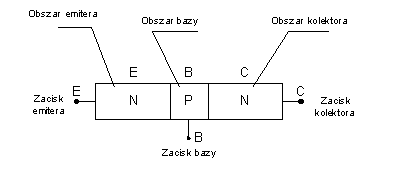
\includegraphics[scale=0.8]{obrazy/tranzystory/budtranbip.png}
\caption{Budowa tranzystora bipolarnego (NPN)}
\end{figure}




\begin{figure}[htbp]
\centering
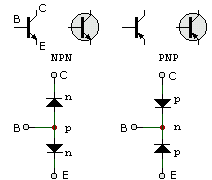
\includegraphics[scale=0.8]{obrazy/tranzystory/tranbipsche.png}
\caption{Diodowe schematy zastępcze tranzystorów bipolarnych}
\label{rys:tranBipDiody}
\end{figure}

Diodowy schemat zastępczy nie odzwierciedla w pełni jego działania, daje jednak pewien pogląd na napięcia występujące między elektrodami.


Główną cechą charakterystyczną tranzystora jest to, że prąd kolektora $I_C$ jest proporcjonalny do prądu bazy $I_B$. Stosunek:
\begin{equation}
\beta = \dfrac{I_C}{I_B}
\end{equation}
zwany jest wielkosygnałowym współczynnikiem wzmocnienia prądowego.

Dalsze rozważania dotyczą tranzystorów typu pnp, w przypadku npn należy zmienić znak wszystkich prądów i napięć na przeciwny.

Po doprowadzeniu $U_{BE}$ i dokonaniu pomiaru $I_C$ w funkcji napięcia wyjściowego $U_{CE}$. Stopniowe zwiększanie napięcia wejściowego daje charakterystykę wyjściową, która została przedstawiona na rys.~\ref{rys:tranBip_ch_przejWyj}.


\begin{figure}[htbp]
\centering
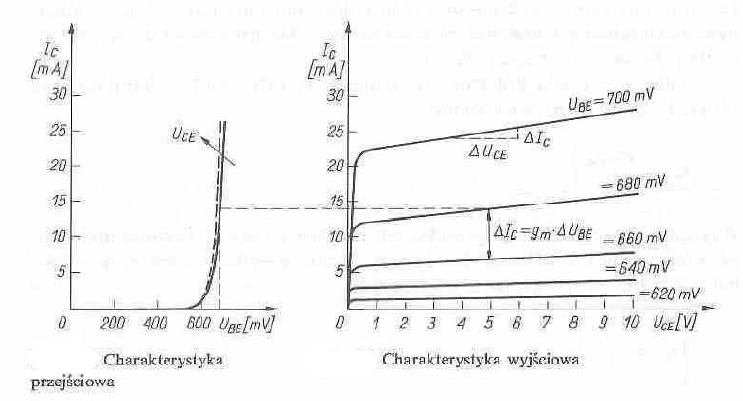
\includegraphics[scale=0.5, width=\linewidth]{obrazy/tranzystory/tranbipcha1.png}
\caption{Charakterystyki: przejściowa i wyjściowa tranzystora bipolarnego}
\label{rys:tranBip_ch_przejWyj}

\end{figure}

Analizując charakterystyka wyjściową można zauważyć, że powyżej pewnego napięcia prąd kolektora prawie nie zależy od $U_{CE}$. Napięcie, przy którym następuje zagięcie charakterystyk nosi nazwę napięcia nasycenia kolektor-emiter $U_{CEsat}$. Drugą ważną właściwością jest fakt, że do wywołania względnie dużej zmiany prądu kolektora wystarczy niewielka zmiana napięcia wejściowego. Ta zmiana, czyli odstęp między charakterystykami, silnie rośnie przy zwiększaniu prądu kolektora. Zmianę tą można dobrze zauważyć na charakterystyce przejściowej z rysunku \ref{rys:tranBip_ch_przejWyj}.

\begin{figure}[htbp]
\centering
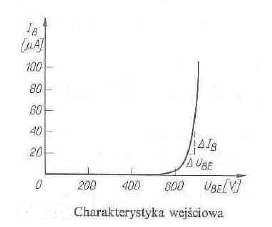
\includegraphics[scale=0.8]{obrazy/tranzystory/tranbipcha2.png}
\caption{Charakterystyka wejściowa tranzystora bipolarnego}
\label{rys:tranBip_chWej}
\end{figure}

Tranzystor w przeciwieństwie do lampy elektronowej nie da się sterować bezprądowo, widać to na powyższej charakterystyce. Wzmocnienie prądowe nie jest stałe, lecz zależy od prądu kolektora.

Prąd kolektora w pierwszym przybliżeniu jest proporcjonalny do prądu bazy. Widać to na rys. \ref{rys:tranBip_Ic(Ib)}. Stosunek $I_C$ do $I_B$ nazywa się statycznym współczynnikiem wzmocnienia prądowego.

\begin{figure}[htbp]
\centering
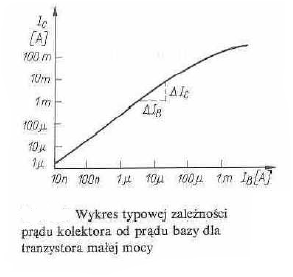
\includegraphics[scale=0.8]{obrazy/tranzystory/tranbipcha3.png}
\caption{Wykres zależności prądu bazy od prądu kolektora}
\label{rys:tranBip_Ic(Ib)}
\end{figure}

\subsubsection{Właściwości tranzystorów bipolarnych}
\begin{itemize}
\item Prąd kolektora jest proporcjonalny do prądu bazy
\item Powyżej pewnego napięcia prąd kolektora prawie nie zależy od $U_{CE}$
\item Do wywołania względnie dużej zmiany prądu kolektora wystarczy niewielka zmiana napięcia wejściowego
\item Tranzystorów bipolarnych nie da się sterować bezprądowo
\item Wzmocnienie prądowe nie jest stałe, lecz zależy od prądu kolektora
\end{itemize}


\subsubsection{Zastosowania}

\subparagraph{Wzmacniacz} – tranzystor pracujący w stanie aktywnym może być wykorzystany do budowy układu będącego wzmacniaczem natężenia prądu elektrycznego. Małe zmiany prądu elektrycznego płynącego w obwodzie bazy powodują duże zmiany prądu płynącego w obwodzie kolektora. W zależności od konstrukcji układu można uzyskać wzmocnienie prądu, napięcia lub obu tych wielkości.


\subparagraph{Przełącznik} – przy pracy tranzystora jako przełącznik wykorzystuje się przejście między stanem nasyconym (tranzystor włączony) a zatkanym (tranzystor wyłączony). Taki tryb pracy tranzystora jest stosowany w niektórych układach impulsowych oraz cyfrowych.

\subsection{Tranzystory unipolarne (polowe)}


\paragraph{Tranzystory unipolarne (polowe)} – są elementami półprzewodnikowymi, trójelektrodowymi, które w przeciwieństwie do normalnych tranzystorów bipolarnych są sterowane polem elektrycznym tzn. bez poboru mocy. Działanie tranzystorów polowych opiera się na sterowaniu przepływem prądu przez kanał za pomocą pola elektrycznego wytwarzanego przez napięcie doprowadzane do elektrody nazywanej bramką. Nie ma tu żadnych przewodzących złącz, więc do bramki nie wpływa ani z niej nie wypływa prąd (za wyjątkiem prądu upływu). Podobnie jak w przypadku tranzystorów bipolarnych, istnieją tranzystory polowe o dwóch różnych rodzajach przewodnictwa: z kanałem typu n (przewodnictwo elektronowe) oraz z kanałem typu p (przewodnictwo dziurowe). Tranzystory polowe mogą być wykonane z dwoma różnymi rodzajami bramek (mamy wiec tranzystory złączowe - JFET i z izolowaną bramką - MOSFET) oraz mogą różnić się sposobem domieszkowania materiału półprzewodnikowego tworzącego kanał (tranzystory ze zubożaniem - rzadko produkowane, i ze wzbogacaniem kanału). 



\subsubsection{Budowa JFET (tranzystora polowego złączowego)}
W tranzystorach JFET, bramka oraz kanał tworzą ze sobą złącze PN lub NP, które zachowuje się jak dioda półprzewodnikowa. Obszar kanału jest słabiej zdomieszkowany (zubożony).
Budowa tranzystora JFET została przedstawiona na rysunku \ref{rys:budowa_jfet}. 
\begin{figure}[htbp]
\centering
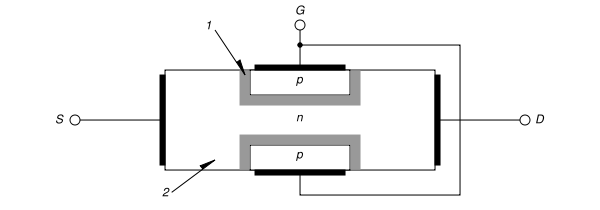
\includegraphics[scale=0.8]{obrazy/tranzystory/tranunijfetbudowa.png}
\caption{Budowa JFET}
\label{rys:budowa_jfet}
\end{figure}


\subsubsection{Budowa MOSFET (tranzystora polowego z izolowaną bramką)}
Najważniejszą cechą tranzystora polowego jest brak prądu bramki. Obszar kanału jest izolowany od bramki cienką warstwą dwutlenku krzemu. Budowa MOSFET'a została ukazana na rysunku \ref{rys:budowa_mosfet}.
\begin{figure}[htbp]
\centering
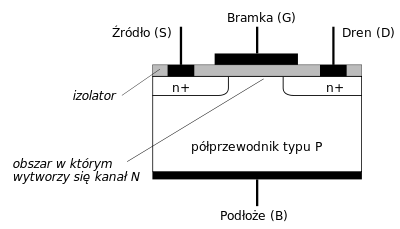
\includegraphics[scale=0.8]{obrazy/tranzystory/tranunimosfetbud.png}
\caption{Budowa MOSFET}
\label{rys:budowa_mosfet}
\end{figure}

\newpage
\subsubsection{Rodzaje tranzystorów polowych}
Klasyfikacja pod względem polaryzacji napięć wejściowych i wyjściowych (ze źródłem dołączonym do masy) została ukazana na rys. \ref{rys:tranUni_klas_we/wy}. Natomiast podział, symbole graficzne, charakterystyki i zastosowania tranzystorów polowych umieszczono w tabeli na końcu niniejszego opracowania.

\begin{figure}[htbp]
\centering
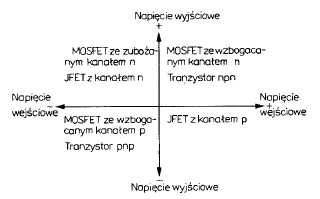
\includegraphics[scale=0.9]{obrazy/tranzystory/tranuniuklad.png}
\caption{Klasyfikacja tranzystorów polowych ze względu na polaryzację napięć we/wy}
\label{rys:tranUni_klas_we/wy}
\end{figure}


\subsubsection{Właściwości tranzystorów polowych}


Jak wynika z powyższych rysunków w normalnym użyciu znajduję się pięć typów tranzystorów polowych. Jednakże, niekoniecznie trzeba pamiętać właściwości każdego z nich gdyż wszystkie zachowują się podobnie. Przykładając jakieś napięcie do bramki (G) sterujemy rezystancją między drenem (D), a źródłem (S). Napięcie sterującym jest napięcie bramka-źródło ($U_{GS}$). Omówione zostaną cechy tranzystora MOSFET z kanałem wzbogacanym typu N.

W tranzystorach JFET bramka i leżący pod nią kanał tworzą złącze półprzewodnikowe. Konieczne jest kontrolowanie polaryzacji napięcia między bramką a kanałem, aby nie dopuścić do spolaryzowania złącza w kierunku przewodzenia - zapobiec przepływowi prądu w obwodzie bramki. Dla przykładu, dla tranzystora typu n dioda będzie przewodzić, jeśli napięcie pomiędzy bramką a źródłem osiągnie wartość +0.6 V. W normalnych warunkach pracy złącze bramka-kanał jest spolaryzowane zaporowo i w obwodzie bramki nie płynie żaden prąd (z wyjątkiem prądu upływności złącza).



\begin{figure}[htbp]
\centering
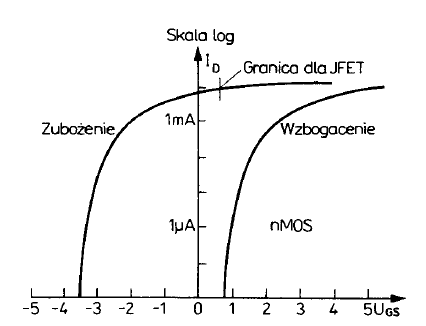
\includegraphics[scale=0.6]{obrazy/tranzystory/tranunicharpor.png}
\caption{Porównanie charakterystyki MOSFET ze zubożeniem i wzbogaceniem}
\label{rys:tranUni_charporow}
\end{figure}



Po pierwsze, dla źródła dołączonego do masy, każdy tranzystor polowy jest wprowadzany w stan przewodzenia (,,włączany'') przez taką zmianę napięcia bramki, aby wartość tego napięcia dążyła do wartości napięcia zasilającego dren w warunkach aktywnej pracy tranzystora.


Po drugie, ze względu na prawie symetryczną konstrukcję tranzystora polowego złączowego, zarówno dren jak i źródło mogą pracować, jako rzeczywiste źródło prądowe (wyjątek stanowią tranzystory MOS mocy, w których podłoże jest połączone ze źródłem wewnątrz obudowy).

Im większa jest wartość napięcia między między bramką a źródłem ($U_{GS}$ tym większa jest wartość prądu drenu ($I_D$).

Podobnie jak tranzystor n-p-n, tranzystor polowy charakteryzuję się dużą przyrostową wartością impedancji obwodu drenu. Przejawia się to stałą wartością prądu drenu, niezależną od wartości napięcia $U_{DS}$ jeśli tylko wartość tego napięcia jest większa od, powiedzmy, 1 V.
Im większa jest wartość napięcia między bramką a źródłem tym większa jest wartość prądu drenu.
W obszarze nasycenia, czyli w normalnym obszarze pracy FET-a prąd drenu nie jest szybkozmienna funkcją napięcia $U_{GS}$. Prąd drenu jest proporcjonalny do $(U_{GS}-U_T)^2$,  gdzie $U_T$ jest napięciem progowym czyli napięciem $U_{GS}$ dla którego zaczyna płynąć prąd drenu.

\paragraph{Podstawowe charakterystyki}


\subparagraph{Przejściowa} – zależność prądu drenu ($I_D$) od napięcia bramka-źródło ($U_{GS}$) przy stałym napięciu dren-źródło ($U_{DS}$). Ukazaną ją na rys. \ref{rys:tranUniIdUgs}.


\begin{figure}[htbp]
\centering
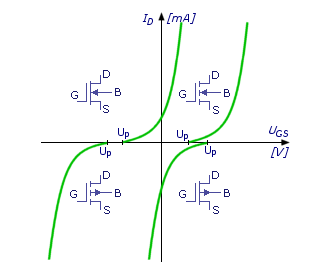
\includegraphics[scale=0.9]{obrazy/tranzystory/tranunichar5.png}
\caption{Charakterystyka przejściowa tranzystorów unipolarnych}
\label{rys:tranUniIdUgs}
\end{figure}


\subparagraph{Wyjściowa} – zależność prądu drenu ($I_D$) od napięcia dren-źródło($U_{DS}$), przy stałym napięciu bramka-źródło ($U_{GS}$). Cały obszar charakterystyki wyjściowej można podzielić na dwie części: obszar nasycenia i obszar nienasycenia (liniowy). Na rysunku \ref{rys:tranUniChWyj} obszary te są rozdzielone niebieską linią, której kształt przypomina parabolę.

\begin{figure}[htbp]
\centering
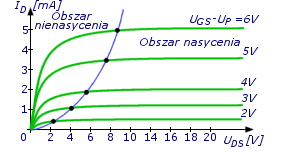
\includegraphics[scale=0.9]{obrazy/tranzystory/tranunichar6.png}
\caption{Charakterystyka wyjściowa tranzystora unipolarnego}
\label{rys:tranUniChWyj}
\end{figure}

W zakresie liniowym (nienasycenia) tranzystor unipolarny zachowuje się jak rezystor półprzewodnikowy. Prąd $I_D$ ze wzrostem napięcia $U_{DS}$ wzrasta w przybliżeniu liniowo.
W zakresie nasycenia napięcie $U_{DS}$ bardzo nieznacznie wpływa na prąd drenu, natomiast bramka zachowuje właściwości sterujące.


\section{Systemy ciągłe i dyskretne: klasyfikacja, opis}

\paragraph{System} można rozumieć jako pewien  blok, który odpowiada na zadany sygnał wejściowy (pobudzenie) jednym lub więcej sygnałami wyjściowym.

\begin{figure}[htbp]
\centering
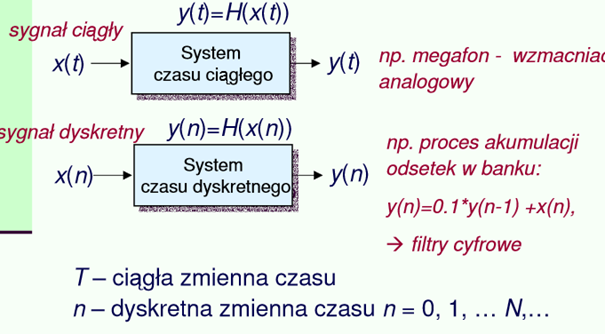
\includegraphics[scale=0.5]{obrazy/ciagle_dyskretne.png}
\end{figure}

\paragraph{Systemy ciągłe} wszystkie sygnały (wejściowe i wyjściowe) są funkcjami ciągłymi w dziedzinie x (np. czasie) i mogą przybierać dowolną wartość z obszaru swojej zmienności. Układy te opisuje się zwykle równaniami różniczkowymi. 

\paragraph{Systemy dyskretne} - układ jest dyskretny, jeżeli przynajmniej jeden jego sygnał ma charakter dyskretny, tzn. przyjmuje tylko określone wartości dla określonych argumentów. Układy takie opisuje się zwykle równaniami różnicowymi. 

W systemie dyskretnym, przetwarzanie
obejmuje operacje arytmetyczne 
przeprowadzane na sygnale wejściowym 
x[n], w wyniku, których na wyjściu systemu otrzymuje się sygnał wyjściowy y[n] w postaci ciągu liczb. W większości przypadków systemy czasu dyskretnego są systemami o jednym wejściu i jednym wyjściu.

Systemy można klasyfikować ze względu na następujące własności:
\begin{itemize}
\item \textbf{Liniowość} - spełnia zasadę superpozycji tj. odpowiedź systemu liniowego na sumę sygnałów wejściowych jest równa sumie odpowiedzi systemu na poszczególne sygnały składowe.
\item \textbf{Przyczynowość} - wyjścia zależą od wejść bieżących i przeszłych, ale nie od wejść przyszłych. Układ taki nie wykazuje reakcji, nim nie nastąpi jego pobudzenie. 
\item \textbf{Stacjonarność} - jeżeli dowolne przesunięcie czasu q dla sygnału wejścia u(t+q) powoduje takie samo przesuniecie dla sygnału wyjścia y(t+q).
\end{itemize}

\paragraph{Właściwości systemów}
\begin{itemize}
\item Addytywność
\[f(x_1(t)+x_2(t))=f(x_1(t))+f(x_2(t))\]
\[f(x_1(n)+x_2(n))=f(x_1(n))+f(x_2(n))\]
\item Jednorodność
\[f(kx(t))=kf(x(t))\]
\[f(kx(n))=kf(x(n))\]
\item Liniowość
\[f(k_1x_1(t)+k_2x_2(t))=k_1f_1(x_1(t))+k_2f_2(x_2(t))\]
\[f(k_1x_1(n)+k_2x_2(n))=k_1f_1(x_1(n))+k_2f_2(x_2(n))\]
\end{itemize}

\subsection{Sygnały}
\paragraph{Sygnał}proces zmian pewnej wielkości fizycznej lub stanu obiektu fizycznego w czasie lub w przestrzeni. Sygnał generalnie przekazuje jakąś informację (tj. jest nośnikiem informacji). Sygnał może być również syntetyzowany do celów komunikacji. 

\subparagraph{Klasyfikacja ze względu na:}
\begin{itemize}
\item \textbf{Dziedzinę} - sygnały ciągłe (określone dla wszystkich $x\in [a,b]$) i dyskretne określone dla wybranych punktów . Poza tymi punktami sygnały są nieokreślone. 
\item \textbf{Przeciwdziedzinę} (zbiór wartości funkcji) Zbiór ten może być ciągły(sygnał ciągły w amplitudzie) lub dyskretny (albo skończony gdy liczba wartości przyjmowanych przez funkcję jest równa N).  
\end{itemize}

\begin{figure}[htbp]
\centering
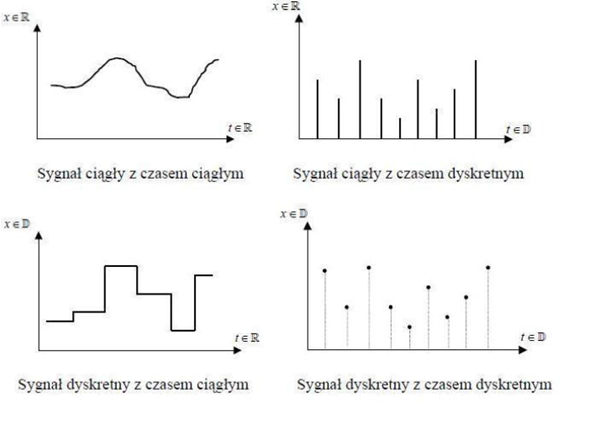
\includegraphics[scale=0.6]{obrazy/wykresy_sygnaly.png}
\caption{Wykresy sygnałów}
\end{figure}

Sygnał dyskretny w  czasie powstaje w wyniku próbkowania sygnałów ciągłych z określonym krokiem próbkowania.

\begin{figure}[htbp]
\centering
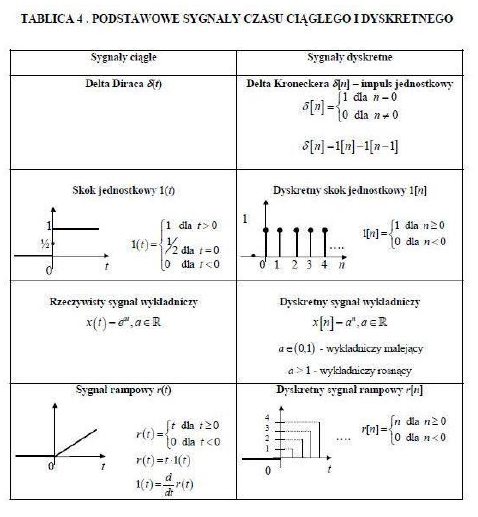
\includegraphics[scale=0.9]{obrazy/podstawowe_sygnaly.png}
\end{figure}

\subsection{Dodatek}
Tematyka systemów jest bardzo rozbudowana - stąd dodatek.

Systemy mogą również być:
\begin{itemize}
\item \textbf{Dynamiczne}
system dynamiczny to taki, w którym zmiana w jednej części wpływa na pozostałe; największy dynamiczny system fizyczny to Wszechświat.
\item \textbf{Statyczne}
system statyczny jest niezmienny w czasie, może być abstrakcyjny lub fizyczny,
\end{itemize}


\begin{figure}[htbp]
\centering
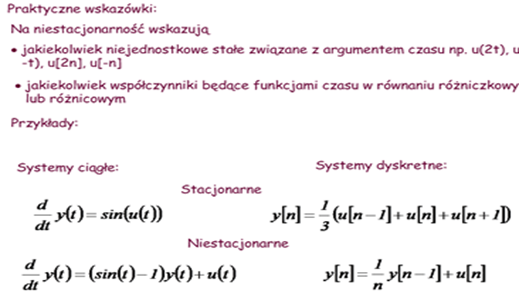
\includegraphics[scale=0.8]{obrazy/slajd.png}
\end{figure}

\paragraph{Systemy nieprzyczynowe} - zwane wyprzedzającymi, to takie, w których wartość sygnału wyjściowego w badanej chwili zależy także od przyszłych wartości sygnału na wejściu. Przykładami takich systemów są:
\begin{itemize}
\item systemy, w których zmienną niezależną nie jest czas (np. systemy cyfrowego przetwarzanie obrazów),
\item systemy w których uśredniamy dane zebrane w pewnym okresie czasu (ceny akcji na giełdzie, dane demograficzne, sygnały meteorologiczne), i w których interesuje nas określenie wolnozmiennych trendów w danych, zawierających także szybkozmienne (często przypadkowe) fluktuacje.
\end{itemize}


\paragraph{System jest odwracalny}, jeżeli jest możliwe znalezienie takiego systemu, który włączony z nim kaskadowo da na wyjściu sygnał wejściowy.

\paragraph{Rozszerzone definicje}
\begin{itemize}
\item \textbf{Sygnał ciągły} – wartości f(x) sygnału są istotne dla każdego argumentu x z pewnego przedziału, np. dla każdej chwili czasu t 
\item \textbf{Sygnał dyskretny} – określony dla dyskretnych wartości argumentu x – gdzie znana jest wartość ilości argumentów x 
\item \textbf{Sygnał analogowy} – jest przebiegiem konkretnej wielkości fizycznej, np. napięcia, natężenie prądu, ciśnienia, temperatury etc. dla konkretnej lub nieskończonej dziedziny argumentu x (np. w czasie). 
\item \textbf{Sygnał cyfrowy} – sygnał określony dla dyskretnych wartości x i f(x). Znaczenie tego terminu może odnosić się do: 
\begin{itemize}
\item wielkości fizycznej, która z natury jest dyskretna (np. liczba błysków lampy w ciągu godziny) 
\item wielkości pierwotnie ciągłej i analogowej, która została spróbkowana i skwantowana (np. sygnał na wyjściu komparatora napięcia kontrolującego pewien proces w określonych chwilach) 
\item każdej reprezentacji jednego z powyższych, w tym (najczęściej) w postaci ciągu liczb zapisanych w pamięci maszyny cyfrowej (np. plik komputerowy typu WAV). 
\end{itemize}
\end{itemize}

\section{Zmienna losowa: właściwości, opis}

\subsection{Zmienne losowe}

\paragraph{Zmienna losowa} X to taka funkcja $X : \Omega \longrightarrow \mathbb{R}$, dla którego dla dowolnego borelowskiego zbioru $B \subset \mathbb{R}$ zbiór:
\begin{equation}
\{\omega : X(\omega) \in B \} = \{X \in B\} \in F,
\end{equation}
tzn. zbiór $X \in B$ jest zdarzeniem losowym.\\\\
Innymi słowy, jest to taka funkcja $X$ na zbiorze zdarzeń elementarnych o wartościach liczbowych, dla której określone są (teoretycznie) prawdopodobieństwa przyjmowania przez $X$ wartości z każdego dowolnego zakresu.\\\\

Zmienna losowa to funkcja przekształcająca wynik eksperymentu losowego na liczbę rzeczywistą. 

Pojęcie zmiennej losowej jest bardzo użyteczne, pozwala na abstrahowanie od postaci przestrzeni zdarzeń a operowanie wyłącznie na liczbach. 

Wyobraźmy sobie rzut kostką sześciościenną. Jest to przykład eksperymentu losowego, czyli eksperymentu, dla którego wiemy jakie sytuacje mogą się wydarzyć, ale nie wiemy która się wydarzy. Możliwe wyniki eksperymentu są najróżniejsze, np. kostka będzie turlała się przez 2 minuty i wypadnie sześć oczek, kostka spadnie ze stołu i wypadnie jedno oczko itp. 

Zmienna losowa to funkcja przedstawiająca wynik eksperymentu w postaci liczby rzeczywistej. Rozważając eksperyment rzutu kostką nie jest dla nas istotne co działo się z kostką, istotne jest jedynie ile oczek wypadło. Dlatego naturalnym wyborem zmiennej losowej jest funkcja określająca liczbę oczek które wypadły w wyniku rzutu kostką. \\\\
Typy zmiennych losowych:
\begin{itemize}
\item \textbf{ciągła} - zmienna przyjmuje dowolne wartości z określonego przedziału (w szczególności cały zbiór liczb rzeczywistych),
\item \textbf{skokowa (dyskretna)} - zmienna przyjmuje dowolne wartości ze zbioru przeliczalnego (np. zbiór liczb całkowitych z określonego przedziału),
\item \textbf{osobliwa} - zmienna losowa, której rozkład skupiony jest na nieprzeliczalnym zbiorze o długości 0 (np. na zbiorze Cantora), tzn. prawdopodobieństwo tego, ze zmienna ta przyjmuje wartość z tego zbioru, wynosi 1, przy czym $P(X = x) = 0$ dla każdego $x \in \mathbb{R}$,
\item dowolna zmienna losowa albo jest jednego z trzech powyższych typów, albo ma rozkład \textbf{mieszany} składający się z rozkładów tych typów.
\end{itemize}

\subsection{Dystrybuanta i jej własności}
\paragraph{Dystrybuanta} zmiennej losowej X  jest to funkcja zdefiniowana następująco:
\begin{equation}
F(x) = P(X \le x).
\end{equation}
(czytamy: ,,Dystrybuanta dla konkretnej wartości zmiennej losowej tj. dla X=x ) jest równa prawdopodobieństwu tego, że zmienna losowa X będzie przyjmowała wartości nie większe niż konkretna wartość  x''.)

Własności dystrybuanty:
\begin{enumerate}
\item $0 \le F(x) \le 1$ dla każdego $x \in \mathbb{R}$,
\item $F(x)$ jest niemalejąca,
\item jest lewostronnie ciągła,
\item $\lim_{x \to - \infty} F(x) = 0, ~~\lim_{x \to + \infty} F(x) = 1.$
\end{enumerate}
\medskip
Dystrybuanta zmiennej losowej \emph{ciągłej} $X$ jest to funkcja podana wzorem:
\begin{equation}
F(x) = P(X < x) = \int_{-\infty}^{x} f(x)~dx.
\end{equation}
\medskip
Dystrybuanta zmiennej losowej \emph{skokowej} X jest to funkcja podana wzorem:
\begin{equation}
F(x)=\sum_{x_i < p_i}^{} p_i.
\end{equation}

\subsection{Funkcja gęstości}

\paragraph{Funkcja gęstości zmiennej losowej ciągłej} to funkcja $f(x)$ okreslona na zbiorze liczb rzeczywistych i spełniająca następujące warunki:

\begin{enumerate}
\item $f(x) \ge 0$ - jest określona nieujemnie,
\item $ \int_{-\infty}^{+ \infty} f(x)~dx = 1$.
\end{enumerate}

\paragraph{Mediana} $M$ to taka wartość zmiennej losowej $x$ dla której dystrybuanta wynosi 1/2.
\begin{equation}
F(x_{0.5}) = P(x < x_{0.5}) = 0.5
\end{equation}


Gęstość prawdopodobieństwa to szansa przyjęcia konkretnej wartości
przez zmienną losową. Dystrybuanta to szansa przyjęcia przez zmienną
losową wartości nie większej od argumentu.

\subsection{Podstawowe parametry rozkładu zmiennej losowej}
\paragraph{Wartość oczekiwana} $E(X)$ (nadzieja matematyczna)
\begin{equation}
E(x) = m.
\end{equation}
Wartość $m$ jest to taka wartość zmiennej losowej $X$, wokół której skupiają się
wyniki wielokrotnych realizacji tej zmiennej. Innymi słowy, oczekuje się (ma
się nadzieje), że wielokrotne realizacje zmiennej losowej $X$ będą skupiały się
wokół liczby $m$. Wartość oczekiwana należy do miar położenia. \\\\
Dla zmiennych losowych \textbf{ciągłych} wzór wygląda następująco:
\begin{equation}
E(x) = \int_{-\infty}^{+ \infty} xf(x)~dx.
\end{equation}
Dla zmiennych losowych \textbf{dyskretnych} wzór wygląda następująco:
\begin{equation}
E(x) = \sum_{i=1}^{n} p_i \cdot x_i.
\end{equation}
\medskip
\paragraph{Wariancja} należy do miar rozproszenia. Można ją wyliczyć wykorzystując wzór:
\begin{equation}
V(x) = E[X - E(X)]^2 = E(X^2)-E(X)^2
\end{equation}
\medskip

\paragraph{Odchylenie standardowe} informuje jak szeroko wartości jakiejś wielkości są rozrzucone wokół jej średniej. 
\begin{equation}
\sigma = \sqrt{V(x)}.
\end{equation}



\section{Ciągła, dyskretna i szybka transformata Fouriera, widmo sygnału}

W dziedzinie przetwarzania sygnałów \textbf{transformacja} Fouriera używana jest do przetworzenia funkcji $x(t)$ ciągłej lub dyskretnej w dziedzinie czasu na funkcję $X(s)$ ciągłą lub dyskretną w dziedzinie częstotliwości. Ocena wyrażenia $X(s)$ pozwala określić zawartość częstotliwościową dowolnego sygnału. 

\subsection{Ciągła transformata Fouriera}
\paragraph{Transformata Fouriera} - wynik operatora liniowego (czyli jednorodny [$ cf(x) = f(cx) $] i addytywny [$f(a+b)=f(a)+f(b)$] ) jakim jest \textbf{transformacja} Fouriera. Dzięki liniowości możemy transformować sygnały rzeczywiste, w innym przypadku byłyby to jedynie sygnały zawierające pojedynczy przebieg sinusoidalny.

Dla funkcji $f(x)$ transformatę Fouriera definiujemy następująco:
$$ F(s) = \int\limits_{-\infty}^{+\infty} f(x)\ e^{- 2\pi i x s}\,dx, $$

a transformację odwrotną

$$ f(x) = \int\limits_{-\infty}^{+\infty} F(s)\ e^{2\pi i x s}\,ds. $$

\subsection{Dyskretna transformata Fouriera (DFT)}
W praktyce pomiary pozwalają otrzymać dane o charakterze dyskretnym, stąd też zdefiniowana jest dyskretna transformata Fouriera (dyskretne przekształcenie Fouriera, DFT), używana w cyfrowym przetwarzaniu sygnałów:

\[ X(m)= \sum_{n=0}^{N-1}{x(n) e^{- \frac{2 \pi i n m}{N}}}, \ 0 \le k \le N-1, \]
gdzie:\\
x(n) - dyskretny ciąg wartości ciągłej zmiennej x(t), spróbkowanej w dziedzinie czasu, \\
N – liczba próbek wejściowych w dziedzinie czasu. \\\\
DFT wyznacza zawartość widmową sygnału wejściowego w $N$ równomiernie rozłożonych punktach na osi częstotliwości. $N$ określa ile próbek wejściowych jest wymaganych do policzenia DFT, jaka jest rozdzielczość wyników w dziedzinie częstotliwości (odległość pomiędzy prążkami w Hz) oraz jaki jest czas przetwarzania wymagany do obliczenia N-punktowej DFT. Ze wzoru na DFT wynika bowiem, iż złożoność obliczeniowa algorytmu wynosi $ O(n^2) $ (to dużo).

\paragraph{DFT}
\begin{itemize}
	\item Jest procedurą matematyczną używaną do wyznaczenia zawartości harmonicznej lub częstotliwościowej sygnału dyskretnego.
	\item Dokładne wartości częstotliwości analizowanych przebiegów (czyli wartości prążków na osi OX) zależą od częstotliwości próbkowania $ f_s $ i liczby próbek $N$. Przykładowo dla sygnału próbkowanego z $ f_s = $ 500~Hz  i 16-punktowej DFT, podstawowa częstotliwość sinusoid wynosi $ fs/N=$ 31.25 Hz. Czyli na otrzymanym wykresie wyznaczone są wartości prążków o częstotliwościach analizy: 0 Hz, 31.25, 62.6, 93.75 … 468.75~Hz.
	\item Wyjściowe wartości amplitud prążków DFT są równe amplitudzie wejściowej danej składowej (sinusoidy) * N/2.
	\item Jeżeli ciąg wejściowy $ x(n) $ jest rzeczywisty, to zespolone wartości wyjściowe DFT dla argumentów $ m \ge (N/2) $ są nadmiarowe w stosunku do wartości wyjściowych dla argumentów od $ m = 0 $ do $ m = (N/2)-1 $. \textit{m}-ta wartość wyjściowa DFT będzie miała taką samą amplitudę jak $(N-m)$-ta wartość wyjściowa DFT. Kąt fazowy $m$-tej wartości będzie równy kątowi fazowemu $(N-m)$-tej wartości wyjściowej DFT, ze znakiem ujemnym. \\\\
	Jeżeli ciąg wyjściowy DFT jest rzeczywisty, to $X(m)$ jest sprzężeniem $X(Nm)$, lub:
$$ X(m) = X^*(N-m) $$
gdzie $ ^* $ oznacza sprzężenie.
\end{itemize}

\paragraph{Podsumowanie}
\begin{itemize}
	\item Każdy człon wyjściowy DFT jest sumą iloczynów wejściowego ciągu w dziedzinie czasu z ciągami reprezentującymi przebieg sinusoidalny i cosinusoidalny, ponieważ można napisać wzór na DFT z użyciem współrzędnych prostokątnych:
	$$ X(m)= \sum_{n=0}^{N-1}{x(n) [\cos(\frac{2 \pi n m}{N}) - i \sin(\frac{2 \pi n m}{N})]}.   $$
	\item Dla rzeczywistych sygnałów wejściowych N-punktowa DFT daje w wyniku jedynie N/2 członów niezależnych.
	\item DFT jest operacją liniową.
	\item Amplitudy składowych wyjściowych DFT są wprost proporcjonalne do N,
	\item Rozdzielczość DFT w dziedzinie częstotliwości wynosi $ f_s/N $.
\end{itemize}

\subsection{Przeciek DFT}
Jeżeli sygnał wejściowy zawiera częstotliwość, która nie należy do częstotliwości ze zbioru $ mfs/N $ (czyli jest gdzieś pomiędzy prążkami wynikowymi) to energia tej składowej ujawni się w pewnym stopniu przy wszystkich $N$ wartościach wyjściowych (czyli prążkach).

\begin{figure}[htbp]
	\centering
	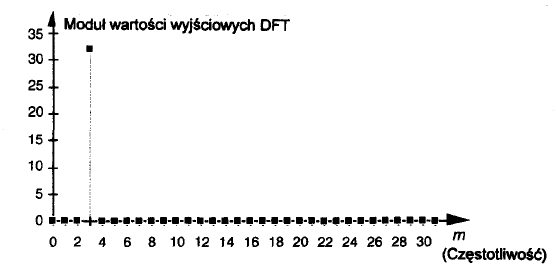
\includegraphics[scale=0.7]{obrazy/fourier/3okresy.png}
	\caption{Wynik 64 punktowej DFT sygnału o częstotliwości 3 okresów w analizowanym oknie 64 próbek}
\end{figure}

\begin{figure}[htbp]
	\centering
	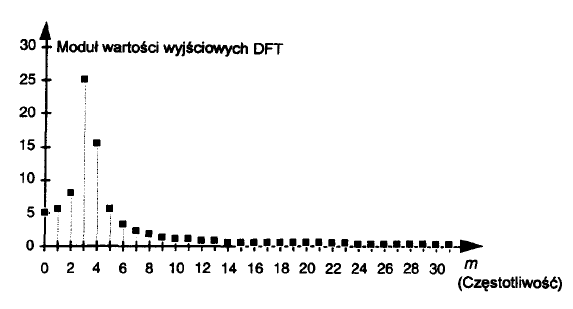
\includegraphics[scale=0.7]{obrazy/fourier/34okresy.png}
	\caption{Wynik DFT dla sygnału o częstotliwości 3.4 okresów w analizowanym oknie 64 próbek }
\end{figure}

Jeszcze prościej: 8 punktowa DFT przy próbkowaniu 8000~Hz daje prążki w punktach 0~Hz, 1000~Hz, 2000~Hz ... 7000~Hz, jak sygnał wejściowy ma składową 1500~Hz to ta ,,rozlewa'' się na wszystkie prążki. 
\paragraph{Przeciek} jest nie do uniknięcia przy wyznaczaniu DFT rzeczywistego ciągu czasowego o skończonej długości.
W celu zminimalizowania skutków przecieku można użyć funkcji okna (jednego z miliona) na wartościach wejściowego ciągu czasowego.
Jak polepszyć rozdzielczość DFT? Zwiększyć $N$, nawet gdy nie mamy więcej próbek, to zawsze można dodać zera i liczyć dla takiego sygnału. 
Poprawa rozdzielczości DFT poprzez uzupełnianie zerami.

\subsection{Szybka transformata Fouriera (FFT)}
Wyznaczenie DFT o tysiącach punktów jest nieefektywne czasowo, tzn. wymaga olbrzymiej mocy obliczeniowej. Z tego powodu w 1965 r. opublikowano artykuł przedstawiający wydajny algorytm implementujący DFT znany dzisiaj jako szybkie przekształcenie Fouriera  - FFT (ang. Fast Fourier Transform). Algorytm przetransformował dziedzinę cyfrowego przetwarzania sygnałów.
Z wielu zaproponowanych algorytmów najpopularniejszym jest algorytm FFT o podstawie 2, tzn. liczba punktów w transformacji wynosi $N=2\cdot k$, gdzie k jest liczbą naturalną.
\paragraph{Zalety FFT o podstawie 2 i metody wykorzystania}
\begin{itemize}
	\item Redukcja ilości mnożeń z N2 do około $N/(2 \cdot \log_2 N)$, dla $N$ = 512 to 200 razy mniej mnożeń zespolonych, dla $N$ = 8192 - redukcja 1000 krotna. 
	\item FFT nie przybliża DFT, ale daje dokładny wynik DFT, z zachowaniem wszystkich właściwości DFT! 
	\item Jeżeli nie mamy wpływu na ilość pobieranych próbek, a nie jest to liczba N2 to należy dodać zera do najbliższej potęgi 2, nigdy nie obcinać.
	\item Poprawianie wyników FFT - do wykrycia sygnałów w obecności szumu, można wykorzystać uśrednianie kolejnych procedur FFT
\end{itemize}

\paragraph{Opis algorytmu\\\\}
Obliczenie N-punktowej FFT można przyspieszyć przez policzenie FFT $N/2$ punktowej, którą można przyspieszyć przez policzenie $N/4$ FFT itd. Za każdym razem obliczenie drugiej połowy FFT jest jedynie kwestią kilku dodawań i przemnożenia przez -1 więc znacząco zmniejsza się ilość operacji (dodatkowo, dodawanie i zmiana znaku jest tańsze od mnożenia)

Warto nauczyć się chociaż jak narysować ,,motylki'' FFT, nie ma sensu tego przepisywać tylko od strony 8 rozdziału 4 z książki Lyonsa.

%\newpage
\subsection{Widmo sygnału}
Określenie składowych częstotliwościowych sygnałów dyskretnych w dziedzinie czasu, dokonywane jest w \textit{dziedzinie częstotliwości}. Zobrazowane $X(m)$ (czyli wartości prążków sygnału) zwane są widmem sygnału.\\
$x(n)$ – ciąg czasowy sygnału,\\
$X(m)$ – ciąg widmowy $X$ zmiennej m.

\begin{figure}[htbp]
	\centering
	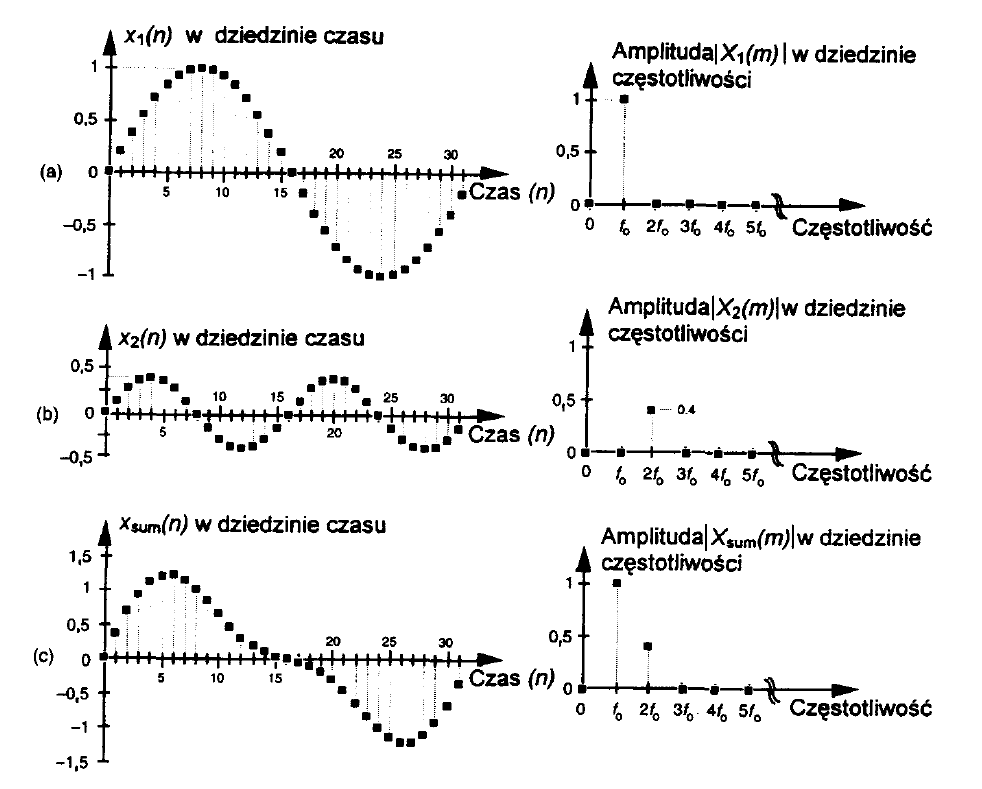
\includegraphics[scale=0.7]{obrazy/fourier/widmo.png}
	\caption{Wynik DFT dla sygnału o częstotliwości 3.4 okresów w analizowanym oknie 64 próbek. }
\end{figure}

\paragraph{Widmo} - przedstawienie sygnału w dziedzinie częstotliwości lub pulsacji, otrzymane przy pomocy transformacji Fouriera.
Z wykresu tego można przykładowo odczytać, jakie składowe harmoniczne wchodzą w skład danego sygnału, czy sygnał ma ograniczone pasmo, jaka jest szerokość jego pasma, czy zawiera składowe wolnozmienne (o małych częstotliwościach) oraz szybkozmienne (o wielkich częstotliwościach). 

Ponieważ transformata Fouriera  $ F(j \omega) $ jest w ogólności funkcją o wartościach zespolonych, zatem przy wykonywaniu wykresów widma wygodne jest niezależne przedstawianie modułu  $ M(\omega) = | F(j \omega) | $ oraz argumentu $ \theta(\omega) = \arg{F(j \omega)} $ . Wykres \textbf{widma amplitudowego}(wykres modułu) pokazuje, jakie są amplitudy składowych widmowych sygnału o różnych częstotliwościach. Wykres \textbf{widma fazowego} (wykres argumentu) pokazuje, jakie są fazy tych składowych.
\section{Modulacje analogowe i cyfrowe}
\paragraph{Modulacja} - celowa lub samorzutna zmiana parametrów sygnału. \\

Na wyjściu źródła informacji sygnał oryginalny jest przeważnie dolnopasmowy. Jednak kanały radiowe i telekomunikacyjne są zawsze środkowoprzepustowe. Aby zamienić sygnał oryginalny na sygnał środkowopasmowy musimy zastosować metodę zwaną modulacją. Modulacja jest to uzmiennienie standardowego przebiegu x(t) nazywanego sygnałem lub falą nośną przez sygnał z(t) zwany sygnałem modulującym. W wyniku tego jako sygnał wyjściowy uzyskujemy sygnał zmodulowany y(t). Schemat blokowy procesu modulacji został przedstawiony na rysunku \ref{rys:modulacja_blok}. Inaczej mówiąc modulacja to zmiana parametrów fali nośnej, która może być np. sinusoidalna lub prostokątna. W przypadku modulowania fal sinusoidalnych zmianom może ulegać amplituda, częstotliwość lub faza. Natomiast dla fal prostokątnych szerokość, amplituda lub ilość impulsów. W zależności od charakteru zmian parametru modulowanego rozróżniamy modulacje analogowe (zmiany o charakterze ciągłym) oraz cyfrowe (zmiany o charakterze skokowym).
\subsection{Modulacje analogowe}

\begin{figure}[htbp]
\centering
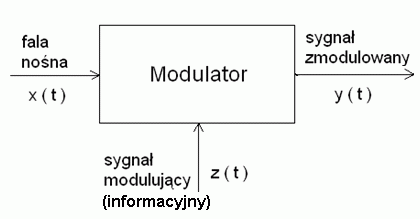
\includegraphics[scale=0.7]{obrazy/modulacja_blok.png}
\caption{Schemat blokowy układu modulacji}
\label{rys:modulacja_blok}
\end{figure}

\paragraph{Modulacja amplitudy AM} (ang. Amplitude Modulation) ma miejsce, gdy w procesie modulacji następują zmiany amplitudy sygnału nośnego proporcjonalne do chwilowej wartości sygnału modulującego. Uzyskujemy ją poprzez zmianę parametru sygnału o częstotliwości nośnej. W tym przypadku jest to amplituda sygnału nośnego Yo, która zmienia się pod wpływem sygnału modulującego z(t). Uzyskujemy w ten sposób sygnał zmodulowany nadający się np. do transmisji drogą radiową. Proces modulacji jest realizowany w urządzeniu zwanym modulatorem. Modulację amplitudy AM charakteryzuje współczynnik głębokości modulacji m, zwany często głębokością modulacji. Definiujemy go jako stosunek amplitudy przebiegu modulującego M do amplitudy sygnału nośnego. Podawany jest on zazwyczaj w procentach. 

\begin{equation}
m=M/Y_0.
\end{equation}

\paragraph{Modulacja częstotliwości FM} (ang. Frequency Modulation) ma miejsce, gdy w procesie modulacji zmianie ulega częstotliwość sygnału nośnego x(t) pod wpływem sygnału modulującego z(t). Częstotliwość chwilowa zmienia się według wzoru:

\begin{equation}
f(t)=f_0+k\cdot z(t),
\end{equation}
gdzie : \\
z(t) - przebieg modulujący,\\
k - stała proporcjonalności.\\

Częstotliwość sygnału nośnego $f_n$ zmienia się w pewnym zakresie, a różnica pomiędzy najniższą i najwyższą chwilową wartością częstotliwości fali nośnej nazywana jest dewiacją częstotliwości $\Delta f$. Stosunek dewiacji częstotliwości do częstotliwości sygnału nośnego:

\begin{equation}
 m_f=\dfrac{\Delta f}{f_n}. 
\end{equation}
nazywamy współczynnikiem modulacji częstotliwości lub wskaźnikiem dewiacji częstotliwości. W zależności od wartości wskaźnika rozróżniamy \textbf{szerokopasmową modulację częstotliwości} (wskaźnik większy od jedności) oraz \textbf{wąskopasmową modulację częstotliwości} (wskaźnik mniejszy od jedności).
 
Modulacja FM jest stosowana nie tylko do przesyłania sygnału radiowego w zakresie fal ultrakrótkich, ale również do transmisji sygnału w telewizji satelitarnej i sygnału dźwiękowego w wielu systemach telewizji naziemnej. 

Modulacja częstotliwości FM jest bardzo podobna do modulacji fazy PM. Gdy zmieniamy częstotliwość sygnału nośnego to zmianie ulega również faza. Identycznie odbywa się to w druga stronę, gdy zmieniamy fazę sygnału nośnego, zmianie ulega również jego częstotliwość. Jednak modulacje FM i PM nie są sobie równoważne. Gdy odbiornik FM jest używany do demodulacji sygnału PM sygnał audio jest zniekształcony. Dzieje się tak dlatego, gdyż związek pomiędzy częstotliwością a fazą jest nieliniowy. 

\paragraph{Modulacja fazy PM} (ang. Phase Modulation) ma miejsce, gdy w procesie modulacji zmianie ulega chwilowa wartość fazy sygnału nośnego x(t), która zmienia się zgodnie z zależnością:

\begin{equation}
\Theta (t)=\omega t+k\cdot z(t),
\end{equation}
gdzie: \\
z(t) - przebieg modulujący,\\
k - stała proporcjonalności. \\

Modulacja częstotliwości pozwala na stosowanie prostszych modulatorów i demodulatorów sygnału. Dlatego też modulację fazy stosujemy głównie do transmisji cyfrowej. Charakterystyczny dla modulacji fazy jest współczynnik zwany dewiacją fazy, który definiujemy w następujący sposób:

\begin{equation}
\Delta \phi _{PM}= k\cdot z_{max}.
\end{equation}



\begin{figure}[htbp]
\centering
%\includegraphics[scale=1]{I2C_Master_Slave_PNG.png}
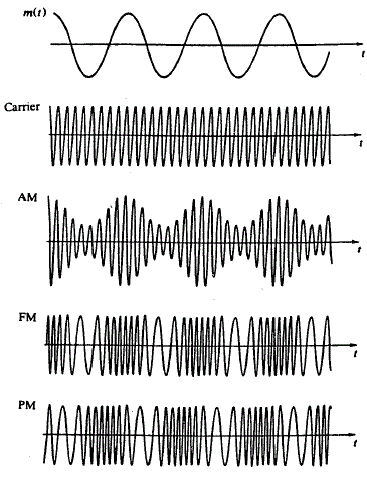
\includegraphics[scale=0.8]{obrazy/modulacje.png}
\caption{Modulacje analogowe}
\label{rys:modulacje}
\end{figure}

 
\subsection{Modulacje cyfrowe}
\paragraph{Modulacja cyfrowa} to proces zmiany analogowego sygnału nośnego przez binarny sygnał modulujący, który z łatwością możemy przesłać, np. drogą radiową. Sygnałem nośnym w modulacji cyfrowej jak i analogowej jest przebieg sinusoidalny, jednak w modulacjach cyfrowych sygnał modulujący to strumień elementów binarnych. Podobnie jak w modulacjach analogowych tak i w cyfrowych zmianom ulega amplituda, częstotliwość lub faza przebiegu nośnego. Ponieważ cyfrowy sygnał modulujący zmienia się skokowo, to zmiany w przebiegu zmodulowanym również są skokowe. Celem modulacji jest dopasowanie właściwości sygnału wyjściowego zmodulowanego do parametrów kanału transmisyjnego.

\paragraph{Modulacja ASK} (ang. Amplitude Shift Keying) zwana kluczowaniem amplitudy ma miejsce, gdy występuje zmiana amplitudy sygnału nośnego w zależności od cyfrowego sygnału modulującego. Proces kluczowania amplitudy jest zbliżony do modulacji amplitudy AM, a w zasadzie jest to szczególny rodzaj modulacji AM. Różnica polega na tym, iż sygnał modulujący jest sygnałem cyfrowym. Cechą charakterystyczną kluczowania amplitudy jest to, że dzięki cyfrowemu sygnałowi modulującemu w czasie trwania stanu wysokiego występuje pełna amplituda sygnału zmodulowanego nato-miast w stanie niskim jest ona wytłumiona. Podobnie jak modulacja AM, kluczowanie amplitudy jest liniowe, czułe na zakłócenia atmosferyczne i zniekształcenia. 

\paragraph{Modulacja FSK}  (ang. Frequency Shift Keying), zwana kluczowaniem częstotliwości, jest szczególnym przypadkiem modulacji częstotliwości FM. Sygnałem modulującym jest sygnał cyfrowy. Modulacja FSK polega na przypisaniu odpowiedniej częstotliwości sygnału nośnego każdemu z dwóch stanów sygnału modulującego. Przejście z jednej częstotliwości może odbywać się z ciągłością fazy lub bez niej. Ta modulacja wyróżnia się stałą amplitudą chwilową, niezależną od sygnału modulującego. Ta właściwość jest bardzo przydatna przy transmisji sygnałów przez kanały, gdzie występują zmiany amplitudy transmitowanego sygnału na skutek nieliniowości tego kanału. Zaletą tej modulacji jest również odporność na zakłócenia impulsowe oraz zniekształcenia tłumieniowe i opóźnieniowe. Dlatego też modulacja FSK jest częściej stosowana niż modulacja ASK. 


\paragraph{Modulacja PSK} (ang. Phase Shift Keying) zwana kluczowaniem fazy to jeden z rodzajów modulacji PM. Ma ona miejsce, gdy przy stałej amplitudzie i częstotliwości harmonicznego sygnału nośnego występuje przesunięcie fazy w zależności od stanu informacji pierwotnej. Sygnały przy modulacji PSK są zawsze transmitowane w systemach koherentnych, czyli faza sygnału nadawanego znana jest po stronie odbiorczej. Podobnie jak w przypadku modulacji FSK, modulacja PSK charakteryzuje się stałą w czasie amplitudą chwilową, co odróżnia ją od modulacji ASK, gdzie amplituda chwilowa zmienia się. Powoduje to większe narażenia na zniekształcenia nieliniowe. 

\paragraph{Modulacja QPSK} (ang. Quadrature Phase Shift Keying) zwana modulacją kwadraturową to jeden z rodzajów modulacji fazy. Może być ona traktowana jako klasyczna modulacja 4 - wartościowa PSK nośnej o amplitudzie A, bądź jako złożenie dwóch dwuwartościowych modulacji amplitudy BASK (ang. Binary Amplitude Shift Keying) o amplitudzie $A/\sqrt{2}$  i ortogonalnych nośnych $\sin 2\pi f_{0}t $  oraz  $\cos 2\pi f_{0}t $. Zastosowano w niej kodowanie na czterech ortogonalnych przesunięciach fazowych sygnału nośnego. Jej zaletą jest zwiększenie efektywności wykorzystania pasma, przy jednoczesnym braku negatywnego wpływu na bitową stopę błędów. Modulację QPSK definiujemy:
\begin{equation}
x=A\cos(2\pi ft + \Theta), ~~~0<t<T,~~i=1,2,3,4~~oraz~~\Theta = \dfrac{\pi(2i-1)}{4}
\end{equation}
Wyjściowe fazy sygnału to Pi/4, 3Pi/4, 5Pi/4, 7Pi/4. Częstotliwość nośnej jest wybierana jako całkowita wielokrotność szybkości nadawania znaku, dlatego faza sygnału jest jedną z wymienionych powyżej faz.

\paragraph{Modulacja MSK}
 (ang. Minimum Shift Keying) jest szczególnym przypadkiem modulacji FSK, gdy częstotliwości f1 i f2 są równe odpowiednio f0 - 1/(4Tb) i f0 + 1/(4Tb). MSK może być również traktowana jako zmodyfikowana forma modulacji OQPSK (ang. Offset Quadrature Phase Shift Keying), w której elementy odpowiadające składowej synfazowej i kwadraturowej są odpowiednio ukształtowane, a następnie wymnożone przez przebiegi nośne. Przez ukształtowanie rozumiemy zastąpienie impulsu prostokątnego impulsem sinusoidalnym. Modulację MSK definiujemy jako:
 
\begin{equation}
s(t)=s_{I}(t)\cos (2\pi f_{0}t)+s_{Q}(t)\sin (2\pi f_{0}t).
\end{equation}

Modulacja MSK zalicza się do klasy modulacji z ciągłą fazą CPM (ang. Continuous Phase Modulation).

%http://atol.am.gdynia.pl/tc/cps2007/cyfrowa.html

\subsubsection{Zastosowania}
\begin{itemize}
\item transmisja danych birarnych w kanale o wąskim paśmie,
\item łączność modemowa, faksowa,
\item łączność radiowa (telemetria, zdalne sterowanie),
\item systemy bezprzewodowe,
\item telefonia cyfrowa (GSM, UMTS, TETRA, ...),
\item łączność satelitarna.
\end{itemize}
\section{Wzmacniacze operacyjne: właściwości i zastosowania}
Materiały: wzmacniacze\_operacyjne.pdf
\section{Mikroprocesory: budowa, zastosowania}
\subsection{Architektury}
\subparagraph{Architektura harwardzka}
W tej architektura pamięć programu przechowująca rozkazy została oddzielona od pamięci danych (dwie różne magistrale). W trakcie pobierania argumentów wykonywanej właśnie instrukcji można równocześnie zacząć pobieranie następnego słowa rozkazowego (pre-fetch).

\subparagraph{Architektura von Neumanna}
Architektura zakłada, że podział przestrzeni adresowej na pamięć programu i pamięć danych jest czysto umowny. W ten sposób jest uproszczony dostęp do obu pamięci, gdyż wykonywany jest za pomocą tych samych instrukcji. Główną wadą jest wydłużenie wykonywania cyklu.

\subparagraph{Architektura super-harwardzka}
Pamięć programu i pamięć danych są oddzielone od siebie, ale wykorzystują one wspólną magistrale: danych i adresową.

\subparagraph{CISC} (ang. Complex Instruction Set Computing) to architektura konwencjonalnych procesorów. Charakteryzuje się ona znaczną liczbą elementarnych rozkazów i trybów adresowania przy niewielkiej liczbie rejestrów uniwersalnych. Jest ona bardzo wolna w porównaniu do RISC-ów. Na tej architekturze były oparte pierwsze procesory z rodziny x86. Dziś w tej rodzinie nie spotka się procesora CISC, ale jest ona zastąpiona przez wewnętrzy RISC. Jednak pozostała zgodnie z zasadą"kompatybilności w tył" mała liczba rejestrów, co jest główną bolączką projektantów procesorów x86.

\subparagraph{RISC} (ang. Reduced Instruction Set Computing/Computer) wywodzi się z Berkeley (1985). Koncepcja tego typu architektury jest oparta na ograniczeniu liczby krótkich (maksymalnie dwusłowowych) rozkazów mających niewiele formatów i trybów adresowania. Procesor RISC posiada wiele rejestrów uniwersalnych (nawet powyżej 100). Działanie procesora przyśpieszają dodatkowe ulepszenia, np. przetwarzanie potokowe, czy pamięć podręczna. Instrukcje wykonująproste operacje, dzięki czemu mogą to robić szybko - każda jednostka wykonawcza jest w stanie wykonać dokładnie jednąinstrukcję w jednym cyklu zegara. Lista instrukcji zawiera tylko kilka rozkazów umożliwiających dostęp do pamięci: załadowanie (load), zapis (store) oraz instrukcje semaforowe. Wszystkie pozostałe rozkazy operują wyłącznie na rejestrach - to również upraszcza budowę układu. Instrukcje kodowane są w prosty sposób - każdy rozkaz ma taką samą długość (np. 32 bity).

\subparagraph{VLIW} (ang. Very Long Instruction Word) – nazwa architektury mikroprocesorów z bardzo długim słowem instrukcji. Obecnie procesory VLIW są oparte na architekturze RISC, zazwyczaj z czterema lub maksymalnie ośmioma jednostkami obliczeniowymi. Po normalnej kompilacji programu, kompilator VLIW porządkuje kod na ścieżki, które wprost nie posiadają jakichkolwiek zależności. Następnie są one dzielone na cztery lub więcej części (jeden dla każdej jednostki obliczeniowej CPU) i pakowane razem w większe instrukcje z dodatkową informacją odnośnie do jednostki, na której ma być wykonywana. Rezultatem tego jest pojedynczy wielki opcode - kod operacji, stąd nazwa ,,Very Long''.

\subsection{Budowa}
Jeśli chodzi o budowę fizyczną, mikroprocesor to nic innego jak krzemowa płytka z milionem tranzystorów, które blokują lub umożliwiają przepływ prądu. Z tranzystorów budowane są bramki logiczne, a te z kolei są łączone w bardziej rozbudowane układy.

\paragraph{ALU} (ang. Arithmetic Logic Unit) - wykonuje podstawowe operacje arytmetyczne (dodawanie, odejmowanie, dzielenie oraz mnożenie oraz logiczne (OR, AND, XOR, NOT) oraz przesunięcia bitowe. ALU współpracuje z roboczym rejestrem zwanym akumulatorem (lub wieloma akumulatorami), który przechowuje jeden z operandów (argumentów) wykonywanej operacji oraz wyniku tej operacji.

\paragraph{CU} (ang. Control Unit) - dekoduje zawartość rejestru rozkazów i generuje odpowiednie sygnały sterujące zapewniające prawidłowy przebieg operacji zdefiniowanej kodem rozkazu.

\paragraph{Rejestry} (ang. Register) - komórki pamięci do przechowywania tymczasowych wyników obliczeń, adresów lokacji w pamięci RAM itp. Rejestry są najszybszym rodzajem pamięci.
\begin{itemize}
\item \textbf{Rejestr instrukcji IR} (ang. Instruction Register) - przechowuje aktualnie wykonywaną instrukcję.
\item\textbf{ Licznik rozkazów PC} (ang. Program Counter) - przechowuje adres w pamięci, gdzie przechowywany jest kolejny rozkaz do pobrania. Rozkazy są przechowywane w postaci kodów binarnych.
\item \textbf{Akumulator A} (ang. Accumulator) - przechowuje argument (operand) do operacji ALU lub wynik operacji.
\item \textbf{Wskaźnik stosu SP} (ang. Stack Pointer) - wskazuje na szczyt stosu (adres ostatniej zapełnionej komórki stosu).
\item \textbf{Rejestr flagowy} - przechowuje informacje dotyczące operacji ALU np. flaga przeniesienia lub pożyczki CF (ang. Carry Flag), flaga parzystości PF (ang. Parity Flag), flaga przepełnienia OF (ang. Overflow Flag) itp.
\end{itemize}

\paragraph{Magistrale} (ang. Bus) - wewnętrzne szyny łączące.
\begin{itemize}
\item \textbf{szyna danych} (ang. data bus) - magistrala komunikacyjna wykorzystywana d przesyłania właściwych danych,
\item \textbf{szyna adresowa} (ang. address bus) - łączy CPU z pamięcią. Określa pod jaki adres mają zostać wysłane dane szyną danych. Szerokość magistrali (liczba linii) określa maksymalną pojemność pamięci systemu (przestrzeń adresową)
\item \textbf{szyna sterująca} (ang. control bus) - zapewnia regulację dostępu do szyny adresowej i szyny danych.
\end{itemize}

\subsection{Mikroprocesor a mikrokontroler}
Na system mikroprocesorowy składa się mikroprocesor, układy wejścia/wyjścia,pamięć programu i danych, szyny adresowe, szyny danych ..., system operacyjny. Mikrokontroler to pojedynczy układ scalony zawierający kompletny system, zdolny do samodzielnego wykonywania operacji arytmetycznych i logicznych oraz do sterowania układami i elementami zewnętrznymi. Typowy uC zawiera CPU, pamięć programu (często FLASH), pamięć danych RAM, układu wejścia/wyjścia, wewnętrzne źródło taktowania, interfejsy komunikacyjne oraz inne układy peryferyjne np. kontroler przerwań, timery, ADC, DAC, DMA.

\subsection{Zastosowania}
\begin{itemize}
\item elektronika przemysłowa - sterowniki PLC,
\item elektronika powszechnego użytku - telefony komórkowe, zegarki, komputery
\item telekomunikacja - routery, switche etc.,
\item technika samochodowa - piloty, sterowniki świateł, lusterek, radia, kontrolery wtrysku,
\item medycyna - ciśnieniomierze, EKG, USG, termometry, mierniki poziomu cukru we krwi,
\item automatyka budynków - sterowniki klimatyzacji i rolet.
\end{itemize}

\section{Sieci komputerowe: budowa, protokoły, zastosowanie}

\textbf{Sieć komputerowa} - wzór wzajemnie połączonych komputerów, które mogą pracować samodzielnie i komunikować się z innymi komputerami.

\subsection{Budowa}

\paragraph{Składniki sieci komputerowych}
\begin{itemize}
\item \textbf{hosty} - komputery wykorzystywane przez użytkowników,
\item \textbf{serwery} - stale działające komputery o dużej mocy obliczeniowej świadczące usługi hostom (udostępnianie plików, baz danych itp.),
\item \textbf{medium transmisyjne} - nośnik informacji (kable miedziane, światłowody lub fale radiowe),
\item \textbf{sprzęt sieciowy} - koncentratory, przełączniki, rutery, karty sieciowe, modemy, punkty dostępu,
\item \textbf{oprogramowanie} - programy komputerowe zainstalowane na urządzeniach sieciowych.
\end{itemize}

\medskip
\paragraph{Model odniesienia OSI} (ang. Open System Interconnection) 
\begin{itemize}
\item \textbf{warstwa aplikacji} - określa w jaki sposób aplikacje działają ze sobą,
\item \textbf{warstwa prezentacji} - dodaje podstawowe formatowanie do prezentacji danych,
\item \textbf{warstwa sesji} - zarządza przebiegiem komunikacji pomiędzy dwoma komputerami,
\item \textbf{warstwa transportowa} - sprawdza poprawność wysyłanych danych,
\item \textbf{warstwa sieci} - adresuje wiadomości wewnątrz i pomiędzy sieciami,
\item \textbf{warstwa łącza danych} - określa sposób uzyskiwania dostępu do fizycznego medium,
\item \textbf{warstwa fizyczna} - przesyła dane przez fizyczne medium.
\end{itemize}

\paragraph{Budowa (topologia)} warunkowana jest przez zastosowanie sieci. Najprostsze komunikowanie się sieci można zrealizować przez jedynie połączenie komputerów, w innych przypadkach używa się urządzeń kierujących ruchem.

\paragraph{Topologia magistrali (szyny, linii)} - połączone jednym, współdzielonym medium.
\subparagraph{Zalety:}
\begin{itemize}
\item Brak koncentratorów/przełączników
\item Awaria węzła nie powoduje paraliżu sieci
\end{itemize}
\subparagraph{Wady:}
\begin{itemize}
\item Awaria kabla powoduje paraliż sieci
\item Ograniczona możliwość rozbudowy
\item Niska przepustowość
\item Obsługuje tylko jeden kanał transmisyjny
\end{itemize}

\paragraph{Topologia gwiazdy} - posiada punkt centralny (switch, koncentrator) i gwiaździście połączone do niego komputery.
\subparagraph{Zalety:}
\begin{itemize}
\item Bardzo łatwa rozbudowa sieci
\item Awaria węzła nie powoduje paraliżu sieci
\item Wysoka przepustowość
\end{itemize}
\subparagraph{Wady:}
\begin{itemize}
\item Ograniczenie odległości stacji roboczej od koncentratora
\item Uszkodzenie koncentratora powoduje całkowity paraliż sieci
\end{itemize}


\begin{figure}[htbp]
\centering
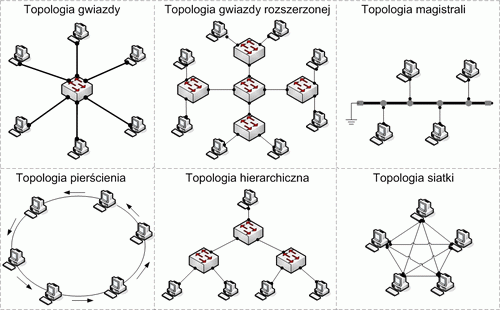
\includegraphics[scale=1]{obrazy/topologie.png}
\caption{Topologie sieci komputerowych}
\label{rys:topologie_sieci_komp}
\end{figure}

\paragraph{Topologia pierścienia} - komputery połączone są za pomocą jednego nośnika informacji w układzie zamkniętym - okablowanie nie ma żadnych zakończeń (tworzy krąg).
\subparagraph{Zalety:}
\begin{itemize}
\item Niskie koszty budowy
\end{itemize}
\subparagraph{Wady:}
\begin{itemize}
\item Niska przepustowość
\item Trudna do rozbudowy
\item Ciężka lokalizacja uszkodzeń
\item Uszkodzenie jednej stacji powoduje paraliż sieci
\end{itemize}

\paragraph{Rozszerzone topologie}
\begin{itemize}
\item \textbf{Topologia siatki}
\item \textbf{Topologia gwiazdy rozszerzonej} – posiada punkt centralny (podobnie do topologii gwiazdy) i punkty poboczne (jedna z częstszych topologii fizycznych Ethernetu)
\item \textbf{Topologia podwójnego pierścienia} – poszczególne elementy są połączone pomiędzy sobą odcinkami tworząc dwa zamknięte pierścienie
\item \textbf{Topologia siatki} – oprócz koniecznych połączeń sieć zawiera połączenia nadmiarowe; rozwiązanie często stosowane w sieciach, w których wymagana jest bezawaryjność
\end{itemize}

\paragraph{Podstawowe urządzenia kierujące ruchem w sieci}
\begin{itemize}
\item Switch -  urządzenie łączące segmenty sieci komputerowej pracujące głównie w drugiej warstwie modelu ISO/OSI (łącza danych), jego zadaniem jest przekazywanie ramki między segmentami sieci z doborem portu przełącznika, na który jest przekazywana.
\item Router - urządzenie sieciowe pracujące w trzeciej warstwie modelu OSI. Służy do łączenia różnych sieci komputerowych. Na podstawie informacji zawartych w pakietach TCP/IP jest w stanie przekazać pakiety z dołączonej do siebie sieci źródłowej do docelowej, rozróżniając ją spośród wielu dołączonych do siebie sieci. Proces kierowania ruchem nosi nazwę trasowania, routingu lub routowania
\end{itemize}




\subsection{Protokoły}

\textbf{Protokół komunikacyjny} - zbiór reguł i kroków postępowania, które są wykonywane podczas komunikacji co najmniej dwóch urządzeń ze sobą.
\medskip 


\subsubsection{Protokoły warstwy aplikacji}

\medskip 
\subparagraph{FTP} (ang. File Transfer Protocol) umożliwia dwukierunkowe przesyłanie plików binarnych i tekstowych, korzysta przy tym z protokołu TCP. FTP działa w oparciu o zasadę klient-serwer i korzystanie z usługi polega na użyciu interaktywnej aplikacji. Technologia FTP zapewnia ochronę stosując hasła dostępu.

\subparagraph{HTTP} (ang. Hypertext Transfer Protocol) odpowiada  za  przesyłanie  dokumentów  hipertekstowych  w  sieci  WWW,  która  jest najszybciej rozwijającą się i najczęściej używaną częścią internetu. Przy jego pomocy przebiega komunikacja między klientami i serwerami sieci Web.

\subparagraph{HTTPS} (ang. HyperText Transfer Protocol Secure) to szyfrowana wersja protokołu HTTP. Zamiast używać w komunikacji klient-serwer niezaszyfrowanego tekstu, szyfruje go za pomocą protokołu SSL. Zapobiega to przechwytywaniu i zmienianiu przesyłanych danych.
HTTPS działa domyślnie na porcie nr 443 w protokole TCP.

\subparagraph{DNS} (ang. Transmission   Control   Protocol) jest systemem tłumaczenia internetowych nazw domenowych na adresy IP. 
System  DNS  jest  rozproszoną  bazą  danych obsługiwaną przez wiele serwerów, z których każdy posiada tylko informacje o domenie, którą zarządza, oraz o adresie serwera nadrzędnego. Na najwyższym poziomie znajdują się tzw. główne serwery nazw(root  level  servers),  które  znajdują  się  w  Stanach  Zjednoczonych  i  podłączone  są  do  szybkich  sieci szkieletowych Internetu. Przechowują one adresy serwerów nazw dla domen najwyższego poziomu, np. .com, .edu, .org, oraz domen krajowych, np. .pl, .de, .uk. Adresy serwerów głównych muszą być znane każdemu  innemu  serwerowi  nazw.  Wewnątrz  każdej  domeny  można  tworzyć  tzw.  subdomeny,  np. wewnątrz domeny .pl utworzono wiele domen regionalnych jak .waw.pl, .lodz.pl itp, oraz funkcjonalnych jak .com.pl, .gov.pl lub .org.pl, należących do firm, organizacji lub osób prywatnych. 

\subparagraph{SMTP} (ang. Simple Mail Transfer Protocol) odpowiada za przesyłanie poczty elektronicznej pomiędzy komputerami pracującymi w sieci.

\subparagraph{POP3} (ang. Post Office Protocol v 3) pozwalający na odbiór poczty elektronicznej ze zdalnego serwera do lokalnego komputera poprzez połączenie TCP/IP. 

\subparagraph{TELNET} (ang. Terminal emulation) - umożliwia użytkownikowi zdalny dostęp do innego komputera: zalogowanie sięw hoście internetowym i wykonywanie poleceń. Wysyłane dane nie są szyfrowane. Aktualnie częściej wykorzystywany jest protokół SSH (ang. Secure SHell) z szyfrowaniem danych.



\subsubsection{Protokoły warstwy transportowej}

\medskip 
\subparagraph{TCP} (ang. Transmission   Control   Protocol)   działa   w   warstwie transportowej   w   \emph{trybie połączeniowym}.  Gwarantuje dostarczenie danych do odbiorcy.  Połączenia  TCP  są  połączeniami  wirtualnymi,  rozpoznawanymi  po  adresach  i portach urządzeń  docelowych  i źródłowych.  Połączenia  takie  charakteryzują  się  możliwościami  sterowania przepływem,    potwierdzaniem    odbioru,    zachowywaniem    kolejności    danych,    kontrolą    błędów    i przeprowadzaniem  retransmisji. Odbiorca po odebraniu danych zobowiązany jest do przesłania do nadawcy potwierdzenia odebrania danych. Jeżeli potwierdzenie nie nadejdzie w określonym czasie, to nadawca wysyła dane ponownie.  Segmenty  TCP  składają  się  z  nagłówka  i  danych.

\subparagraph{UDP} (ang. User   Datagram   Protocol)   działa    w    warstwie    transportowej   w   \emph{trybie bezpołączeniowym}.  Protokół  ten  nie  gwarantuje  dostarczenia  danych  do  odbiorcy.  Jeżeli  pakiet  nie dotrze  do  odbiorcy,  lub  dotrze  uszkodzony,  UDP  nie podejmie żadnych  działań  zmierzających  do retransmisji  danych,  a  zapewnienie  niezawodności  pozostawi  warstwie  wyższej.   Protokół wykorzystywany jest do szybkiego przesyłania danych w niezawodnych sieciach. 




\subsubsection{Protokoły warstwy sieci}

\medskip 
\subparagraph{IP} (ang. Internet Protocol) zapewnia usługę dostarczania pakietów danych z jednego punktu sieci do drugiego. Nie analizuje zawartości pakietu, ale wyszukuje ścieżkę prowadzącą do jego miejsca przeznaczenia. Protokół ten wykorzystuje adresy sieciowe komputerów zwane adresami IP. Są to 32-bitowa liczby zapisywana jako sekwencje czterech ośmiobitowych liczb dziesiętnych (mogących przybierać wartość od 0 do 255), oddzielonych od siebie kropkami. Adres IP dzieli się na dwie części: identyfikator sieciowy (network id) i identyfikator komputera (host id). Istnieje kilka klas adresowych, o różnych długościach obydwu składników. Obowiązujący obecnie sposób adresowania ogranicza liczbę dostępnych adresów, co przy bardzo szybkim rozwoju Internetu jest dla niego istotnym zagrożeniem. W celu ułatwienia zapamiętania adresów wprowadzono nazwy symboliczne, które tłumaczone są na adresy liczbowe przez specjalne komputery w sieci, zwane serwerami DNS.

\subparagraph{ARP} (ang. Address Resolution Protocol) odpytuje wszystkie komputery w sieci, czy maja potrzebny mu adres IP i prosi o przesłanie odpowiadającego mu adresu fizycznego MAC. Aby ograniczyć ruch w sieci budowana jest dynamiczna tablica ARP, w której zapisywane są pary adres IP adres MAC komputerów z którymi został nawiązany kontakt. Tablica ta ma ograniczony rozmiar. Jeśli tablica ARP przepełni się, to jest z niej usuwany najstarszy wpis.

\subsection{Zastosowania}
\medskip 
\begin{itemize}
\item współdzielenie zasobów np. plików, drukarek,
\item komunikacja np. poczta e-mail, telefonia,
\item sieci przemysłowe,
\item bezprzewodowe sieci czujników,
\end{itemize}


\begin{figure}[htbp]
\centering
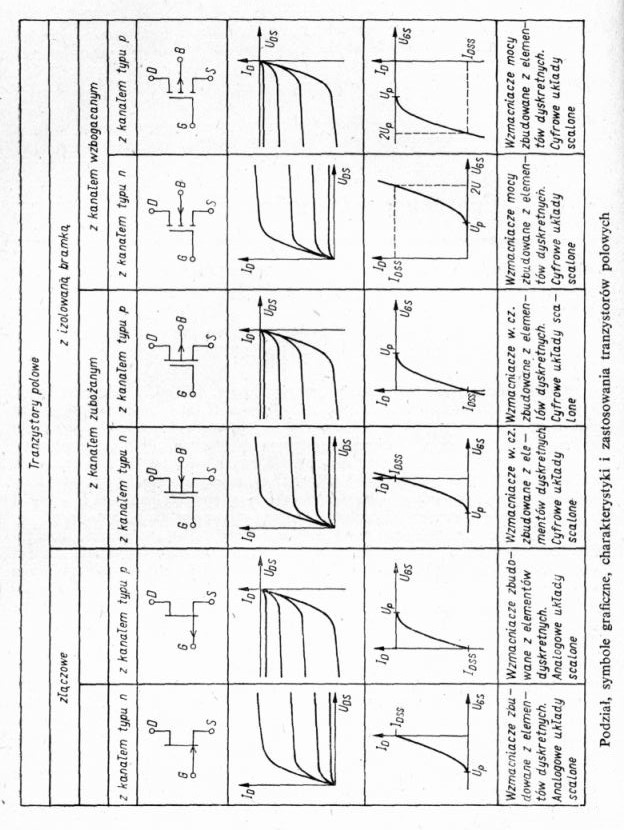
\includegraphics[width=\linewidth]{obrazy/tranzystory/ch-ki_polowe.jpg} 
\end{figure}
\end{document}
